\section{Radionuclide Transport Base Cases}\label{sec:nuclide_base_cases}
\subsection{Basic Transport and Containment Problem Specification}
Basic transport and containment base cases were conducted to verify the 
fundamental behavior of all the radionuclide transport models at each component 
interface. These integration tests neglected thermal transport and capacity 
estimation to simplify the results.  

The problem design includes : 
\begin{itemize}
\item{A source facility providing one waste stream per time step}
\item{An initial capacity of 5 1kg waste streams}
\item{Waste form Components each accepting 1 waste stream} 
\item{Corresponding waste package Components, one per waste form}
\item{A buffer Component}
\item{A far field Component}
\end{itemize}

\subsubsection{Degradation Rate Model}
The Degradation Rate model should not release contaminants if the degradation 
rate is 0. If the degradation rate is nonzero, however, and a fixed maximum 
transport mode is selected, contaminants should become available immediately to 
the adjacent components, traveling quickly across the interfaces. 

To observe these behaviors, four simulations were run to demonstrate that total 
containment resulted from a degradation rate of 0 and that congruent release 
resulted from nonzero degradation rates. A description of these verification 
cases can be found in Table \ref{tab:dr_base}. The 0 degradation rate component was 
different for each of the four cases. This resulted in total containment at the 
Waste Form, Waste Package, Buffer, and Far Field interfaces respectively. 
Results of these base cases can be found in Figures 
\ref{fig:drIwf5} through \ref{fig:drIVff0}.
\FloatBarrier
\begin{table}[htp!]
\centering
\footnotesize{
\begin{tabularx}{\textwidth}{|X|c|c|r|r|}
  \multicolumn{5}{c}{\textbf{Degradation Rate Model No Release Contaminant Transport}}\\
  \hline
  \textbf{Case}  &  \textbf{Component} &  \textbf{Degradation Rate} & \textbf{Expected 100 yrs} & \textbf{Actual 100 yrs}\\
  \textbf{ID}    & \textbf{[Type]} &  \textbf{$[yr^{-1}]$}  &  $[\%]$  & $[\%]$\\
  \hline
  DRI     &  WF    &  0   & 100 & 100\\
          &  WP    &  0.1 & 0 & 0 \\
          &  BUFF  &  0.1 & 0 & 0 \\
          &  FF    &  0.1 & 0 & 0\\
  \hline
  DRII    &  WF    &  0.1 & 0 & 0\\
          &  WP    &  0   & 100 & 100\\
          &  BUFF  &  0.1 & 0 & 0\\
          &  FF    &  0.1 & 0 & 0\\
  \hline
  DRIII   &  WF    &  0.1 & 0 & 0\\
          &  WP    &  0.1 & 0 & 0\\
          &  BUFF  &  0   & 100 & 100\\
          &  FF    &  0.1 & 0 & 0\\
  \hline
  DRIV    &  WF    &  0.1 & 0 & 0\\
          &  WP    &  0.1 & 0 & 0\\
          &  BUFF  &  0.1 & 0 & 0\\
          &  FF    &  0   & 100 & 100\\
  \hline
\end{tabularx}
\caption[Degradation rate model no release problem results.]{Results from demonstration cases for non-release from 0-degradation Degradation Rate modeled Components.}
\label{tab:dr_base}
}
\end{table}


\begin{figure}[ht]
\centering
\includegraphics[width=0.6\textwidth]{./chapters/demonstration/base/drI.eps}
\caption[$^{235}U$ residence. Degradation Rate Waste Form No Release.]{
For Case DRI, in which total containment in the waste form is assumed ($F_{d,wf}=0$), 
$^{235}U$ takes up permanent residence in the waste form component.
}
\label{fig:drIall}
\begin{minipage}[b]{0.45\linewidth}

  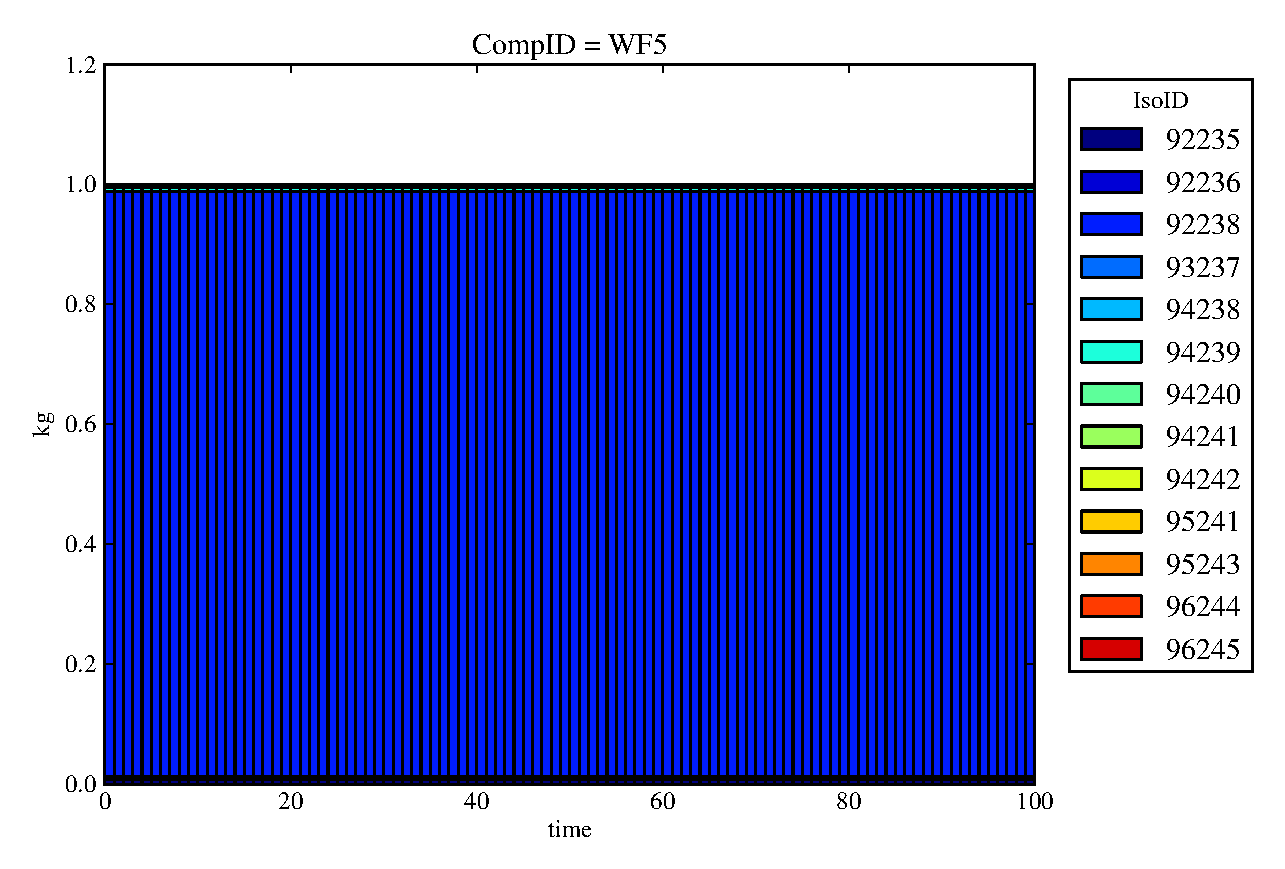
\includegraphics[width=\textwidth]{./chapters/demonstration/base/drI1.eps}
  \caption[DRI Waste Form Contaminants.]{
    Waste Form 5 ($F_d = 0$) never releases material.
    }
  \label{fig:drIwf5}
  
  \includegraphics[width=\textwidth]{./chapters/demonstration/base/drI3.eps}
  \caption[Case DRI Buffer Contaminants]{
    The Buffer, component 7 ($F_d = 0.1$), never recieves material.
    }
  \label{fig:drIbuff}

\end{minipage}
\hspace{0.05\linewidth}
\begin{minipage}[b]{0.45\linewidth}
  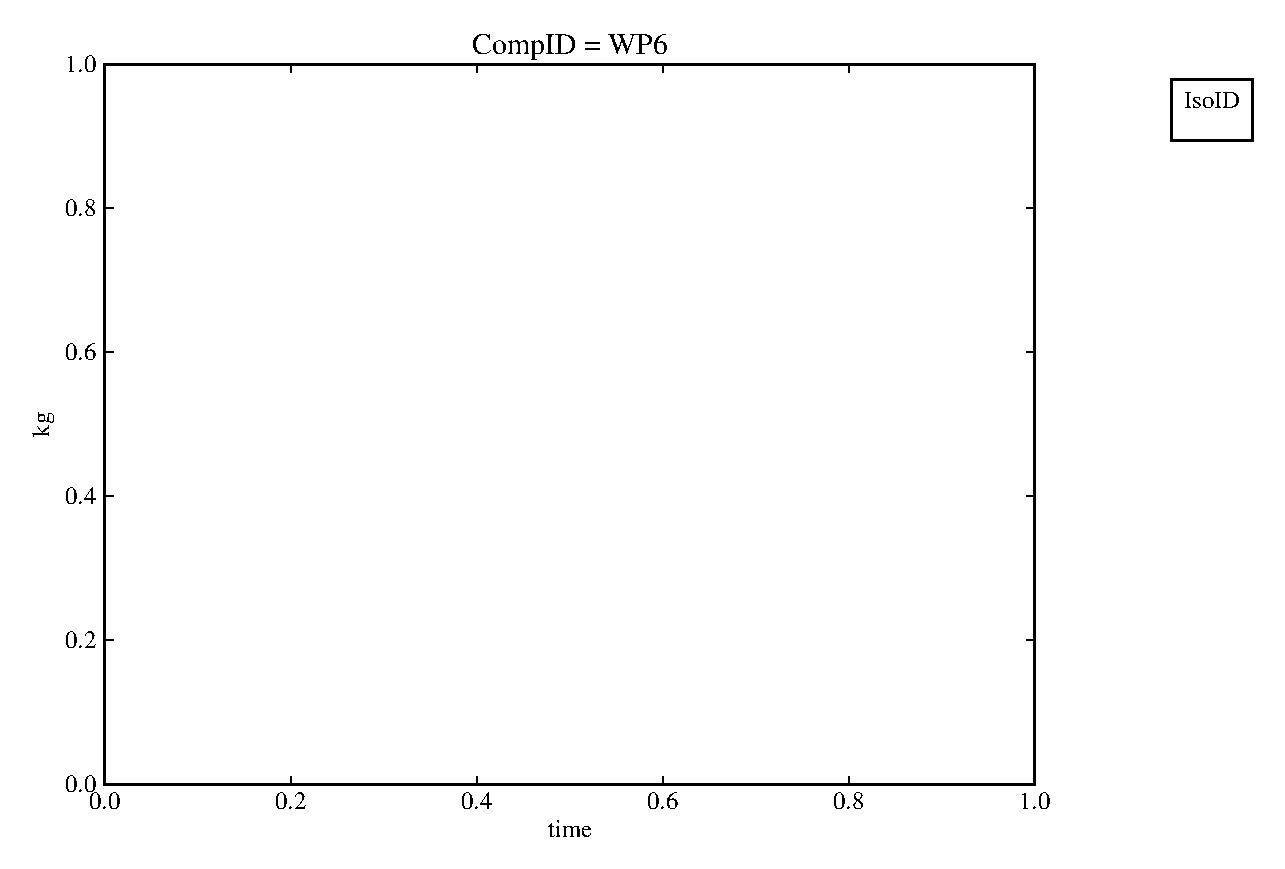
\includegraphics[width=\textwidth]{./chapters/demonstration/base/drI2.eps}
  \caption[Case DRI Waste Package Contaminants.]{ 
    Waste Package 6 ($F_d = 0.1$), never recieves material.
    }
  \label{fig:drIwp6}

  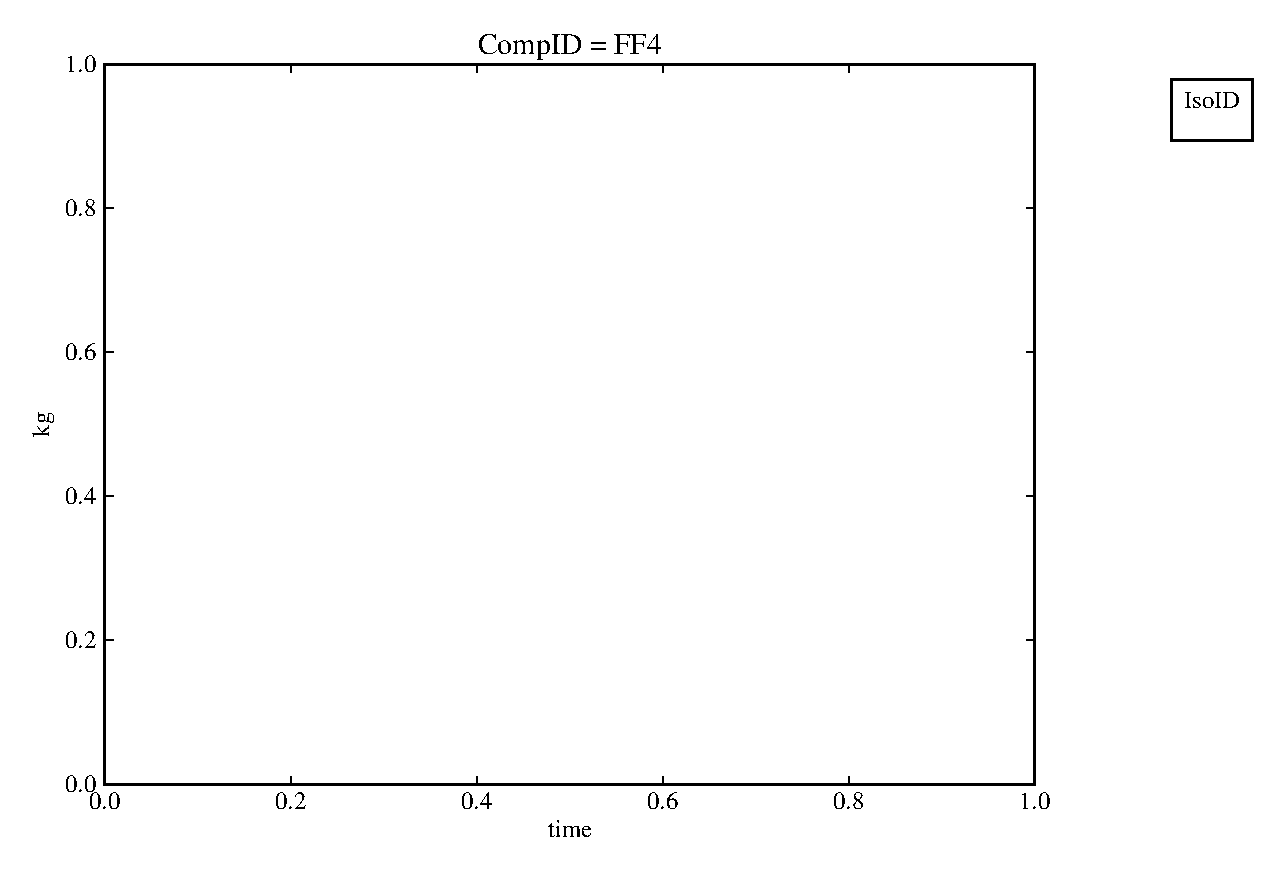
\includegraphics[width=\textwidth]{./chapters/demonstration/base/drI0.eps}
  \caption[Case DRI Far Field Contaminants.]{ 
    The Far Field, component 0 ($F_d = 0.1$), never recieves material.
    }
  \label{fig:drIff0}

  \end{minipage}
\end{figure}
\FloatBarrier



\begin{figure}[ht]
\centering
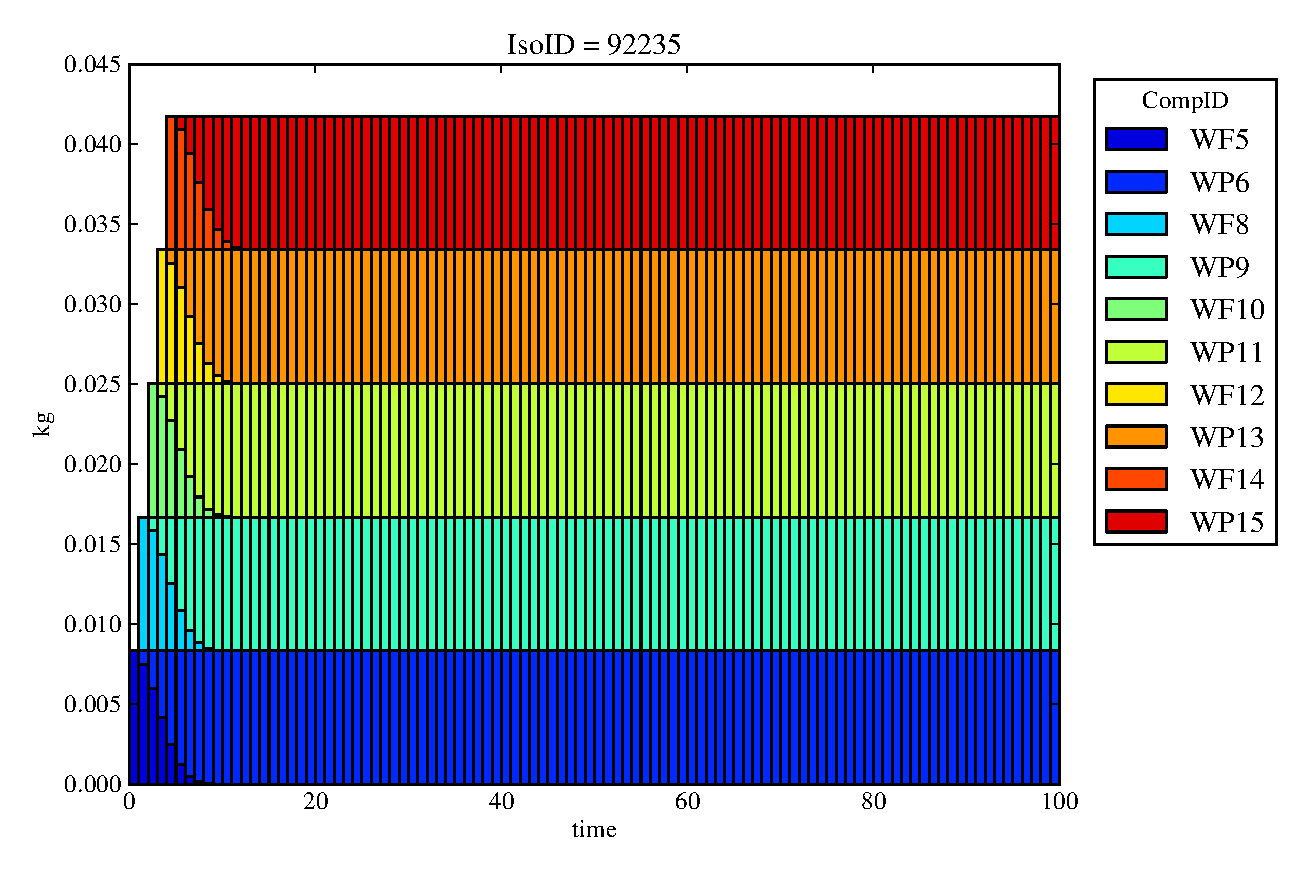
\includegraphics[width=0.6\textwidth]{./chapters/demonstration/base/drII.eps}
\caption[$^{235}U$ residence. Degradation Rate Waste Package No Release.]{
For Case DRII, in which total containment in the waste package is assumed ($F_{d,wp}=0$), 
$^{235}U$ travels through waste forms ($F_d = 0.1$) before 
permanent residence in the waste package components.
}
\label{fig:drIIall}
\begin{minipage}[b]{0.45\linewidth}

  \includegraphics[width=\textwidth]{./chapters/demonstration/base/drII1.eps}
  \caption[DRII Waste Form Contaminants.]{
    Waste Form 5 ($F_d = 0.1$) releases material with degradation. 
    }
  \label{fig:drIIwf5}
  
  \includegraphics[width=\textwidth]{./chapters/demonstration/base/drII3.eps}
  \caption[Case DRII Buffer Contaminants]{
    The Buffer, component 7 ($F_d = 0.1$), never recieves material.
    }
  \label{fig:drIIbuff}

\end{minipage}
\hspace{0.05\linewidth}
\begin{minipage}[b]{0.45\linewidth}
  \includegraphics[width=\textwidth]{./chapters/demonstration/base/drII2.eps}
  \caption[Case DRII Waste Package Contaminants.]{ 
    Waste Package 6 ($F_d = 0$) acheives total containment.
    }
  \label{fig:drIIwp6}

  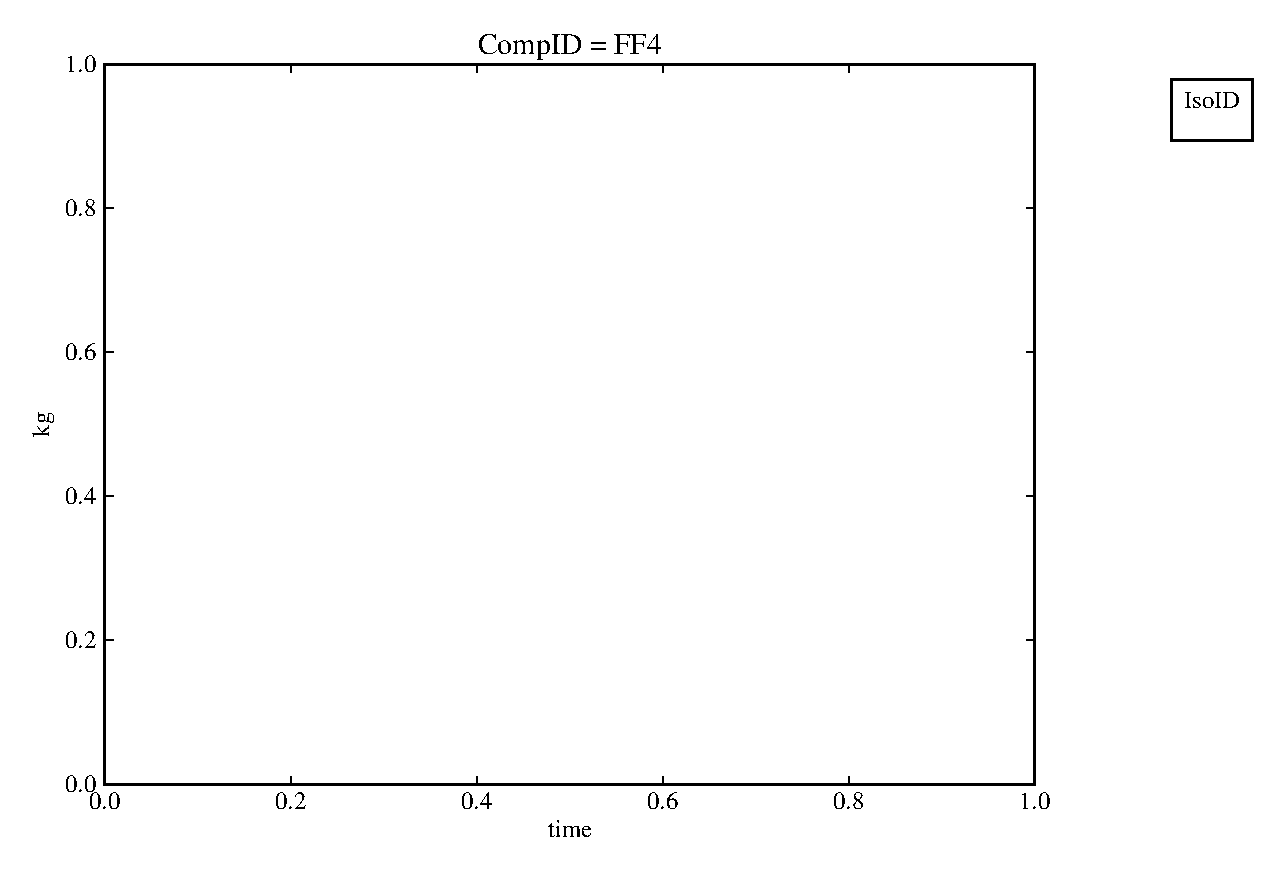
\includegraphics[width=\textwidth]{./chapters/demonstration/base/drII0.eps}
  \caption[Case DRII Far Field Contaminants.]{ 
    The Far Field, component 0 ($F_d = 0.1$), never recieves material.
    }
  \label{fig:drIIff0}


  \end{minipage}
\end{figure}
\FloatBarrier

\begin{figure}[ht]
\centering
\includegraphics[width=0.6\textwidth]{./chapters/demonstration/base/drIII.eps}
\caption[$^{235}U$ residence. Degradation Rate Buffer No Release.]{
For Case DRIII, in which total containment in the buffer is assumed ($F_{d,buffer}=0$), 
$^{235}U$ travels through waste forms and waste package components ($F_d = 0.1$) before 
permanent residence in the buffer component.
}
\label{fig:drIIIall}
\begin{minipage}[b]{0.45\linewidth}

  \includegraphics[width=\textwidth]{./chapters/demonstration/base/drIII1.eps}
  \caption[DRIII Waste Form Contaminants.]{
    Waste Form 5 ($F_d = 0.1$) releases material with degradation. 
    }
  \label{fig:drIIIwf5}
  
  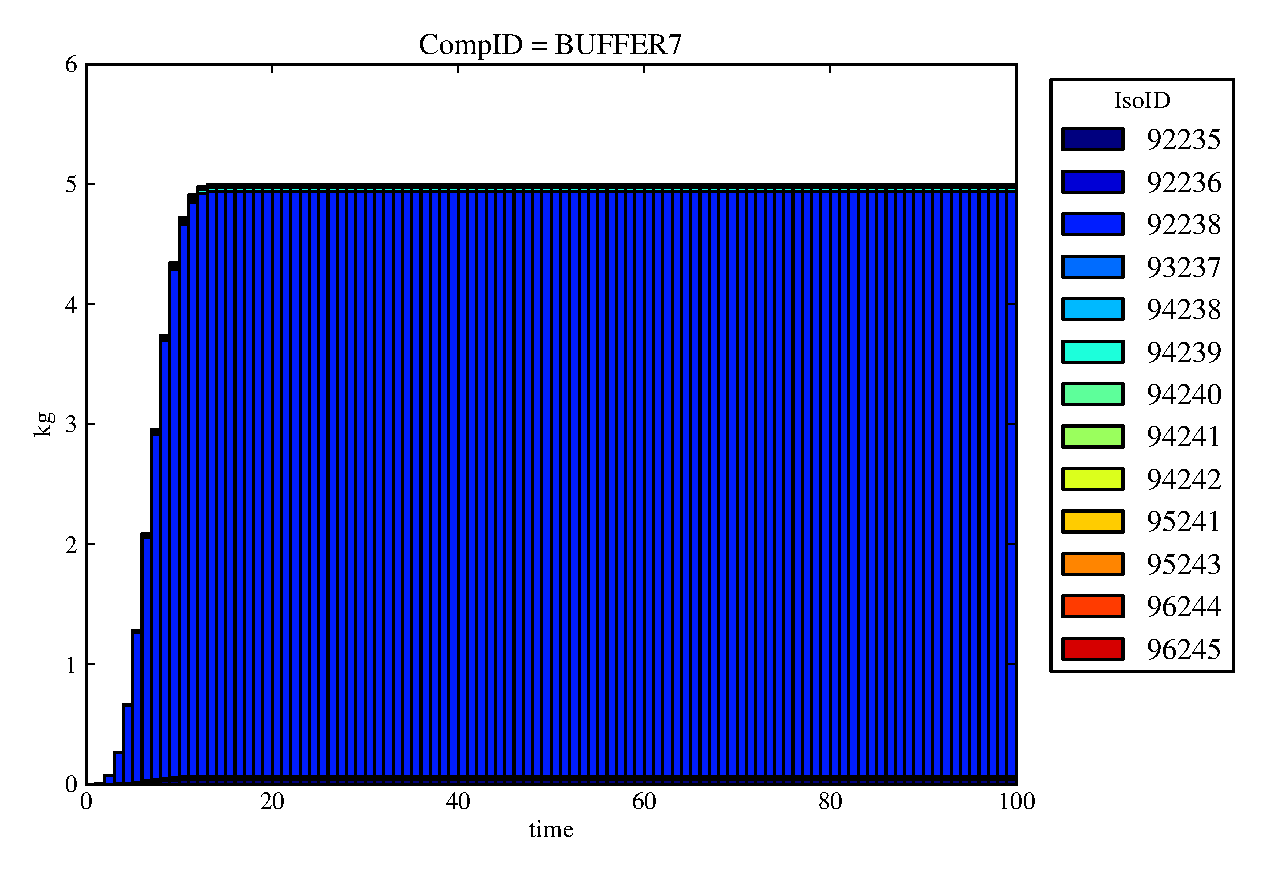
\includegraphics[width=\textwidth]{./chapters/demonstration/base/drIII3.eps}
  \caption[Case DRIII Buffer Contaminants]{
    The Buffer, component 7 ($F_d=0$), acheives total containment.
    }
  \label{fig:drIIIbuff}

\end{minipage}
\hspace{0.05\linewidth}
\begin{minipage}[b]{0.45\linewidth}
  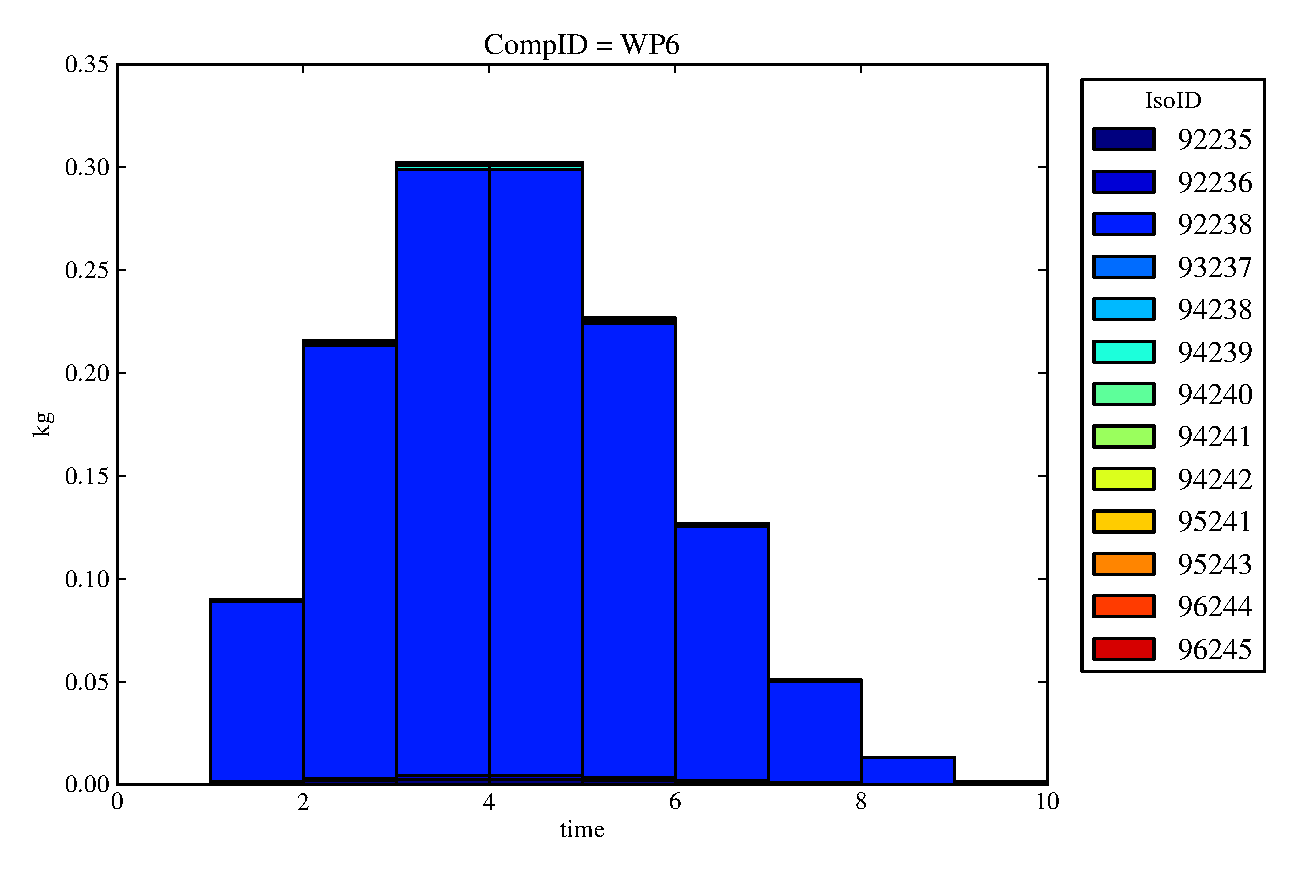
\includegraphics[width=\textwidth]{./chapters/demonstration/base/drIII2.eps}
  \caption[Case DRIII Waste Package Contaminants.]{ 
    Waste Package 6 ($F_d = 0.1$) recieves then releases material. 
    }
  \label{fig:drIIIwp6}

  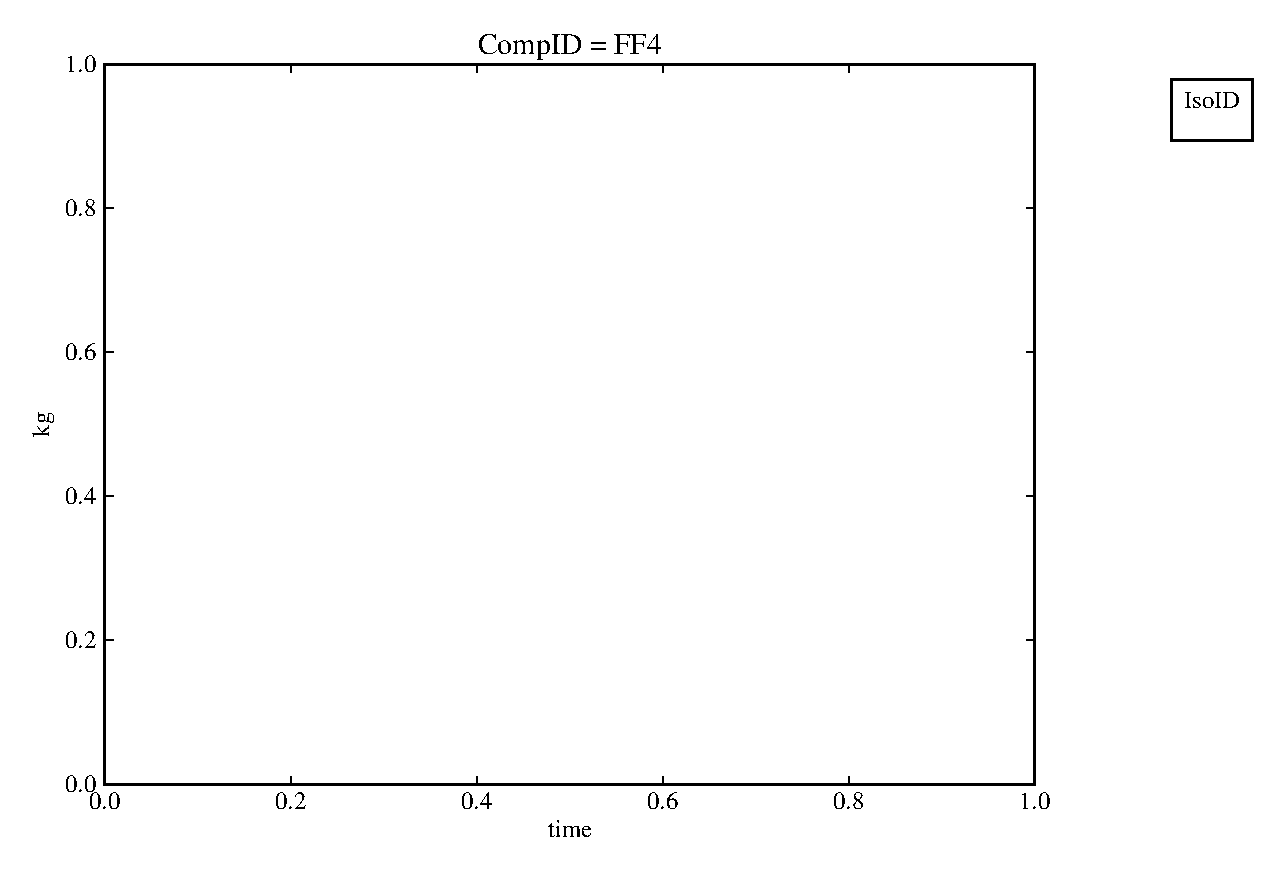
\includegraphics[width=\textwidth]{./chapters/demonstration/base/drIII0.eps}
  \caption[Case DRIII Waste Package Contaminants.]{ 
    The Far Field, component 0 ($F_d = 0.1$), never recieves material.
    }
  \label{fig:drIIIff0}


  \end{minipage}
\end{figure}
\FloatBarrier



\begin{figure}[ht]
\centering
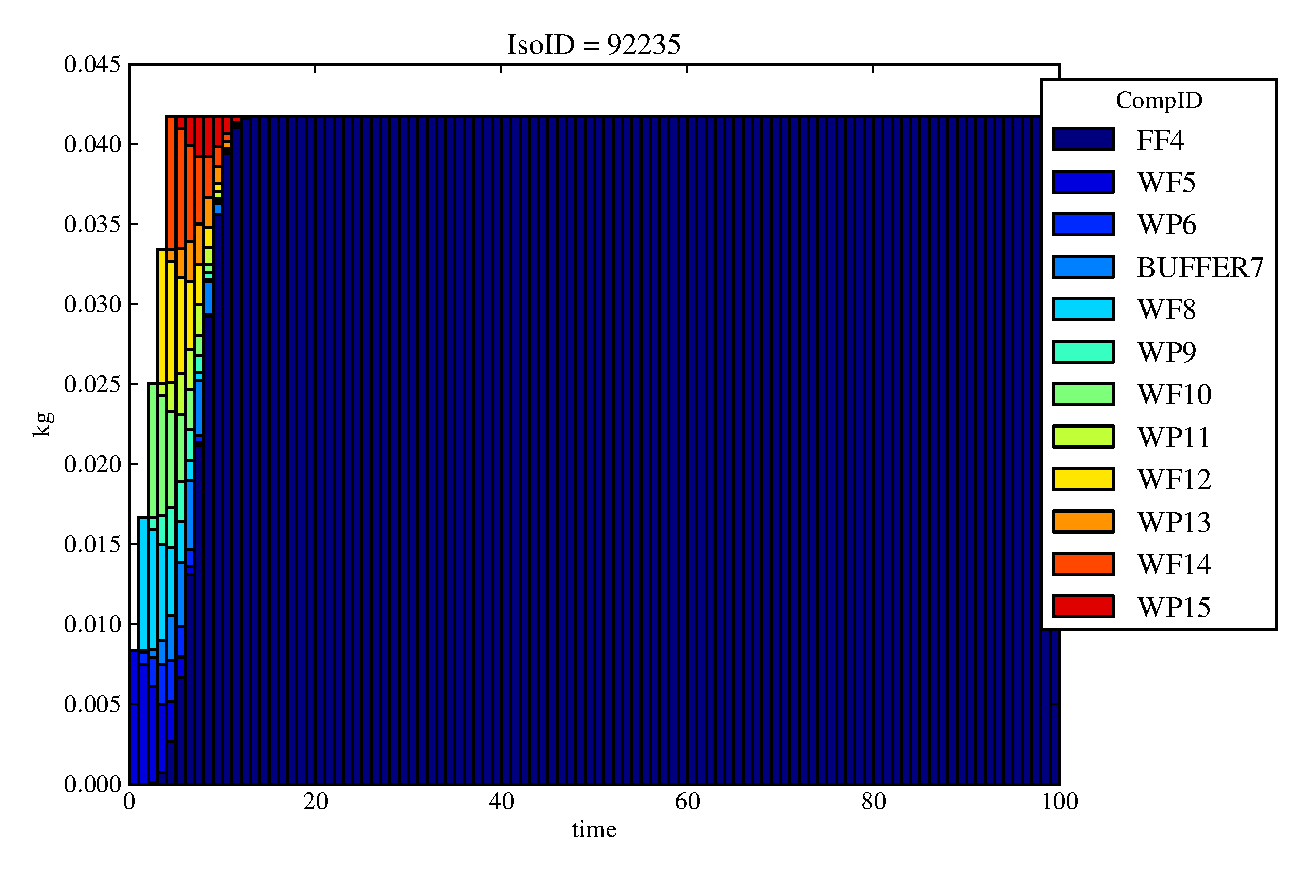
\includegraphics[width=0.6\textwidth]{./chapters/demonstration/base/drIV.eps}
\caption[$^{235}U$ residence. Degradation Rate Buffer No Release.]{
For DRIV case in which total containment in the far field is assumed ($F_{d,ff}=0$), 
$^{235}U$ travels through interior components ($F_d = 0.1$) before 
permanent residence in the far field component.
}
\label{fig:drIVall}
\begin{minipage}[b]{0.45\linewidth}

  \includegraphics[width=\textwidth]{./chapters/demonstration/base/drIV1.eps}
  \caption[DRIII Waste Form Contaminants.]{
    Waste Form 5 ($F_d = 0.1$) releases material with degradation. 
    }
  \label{fig:drIVwf5}
  
  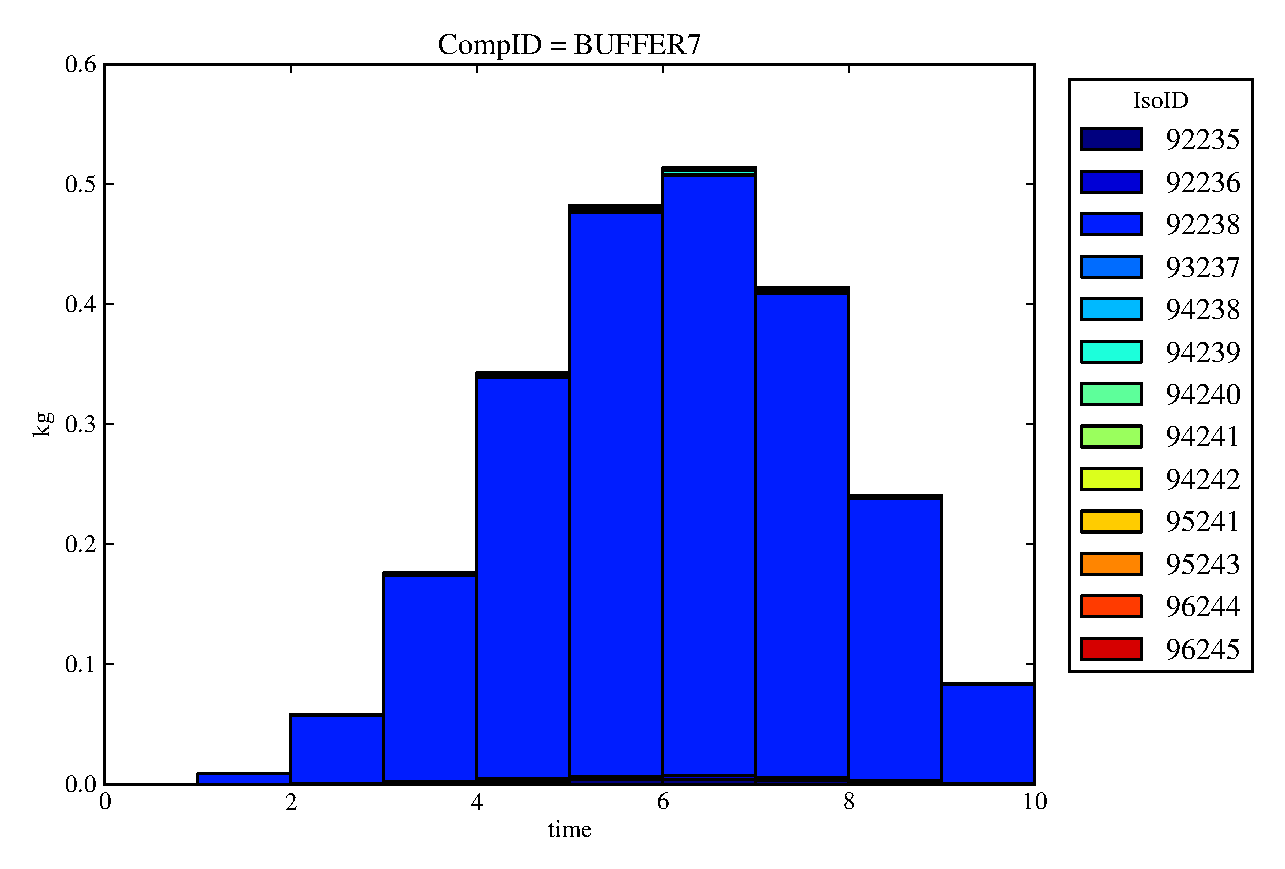
\includegraphics[width=\textwidth]{./chapters/demonstration/base/drIV3.eps}
  \caption[Case DRIII Buffer Contaminants]{
    The Buffer, component 7 ($F_d=0.0$), receives and then releases material.
    }
  \label{fig:drIVbuff}

\end{minipage}
\hspace{0.05\linewidth}
\begin{minipage}[b]{0.45\linewidth}
  \includegraphics[width=\textwidth]{./chapters/demonstration/base/drIV2.eps}
  \caption[Case DRIII Waste Package Contaminants.]{ 
    Waste Package 6 ($F_d = 0.1$) recieves then releases material. 
    }
  \label{fig:drIVwp6}

  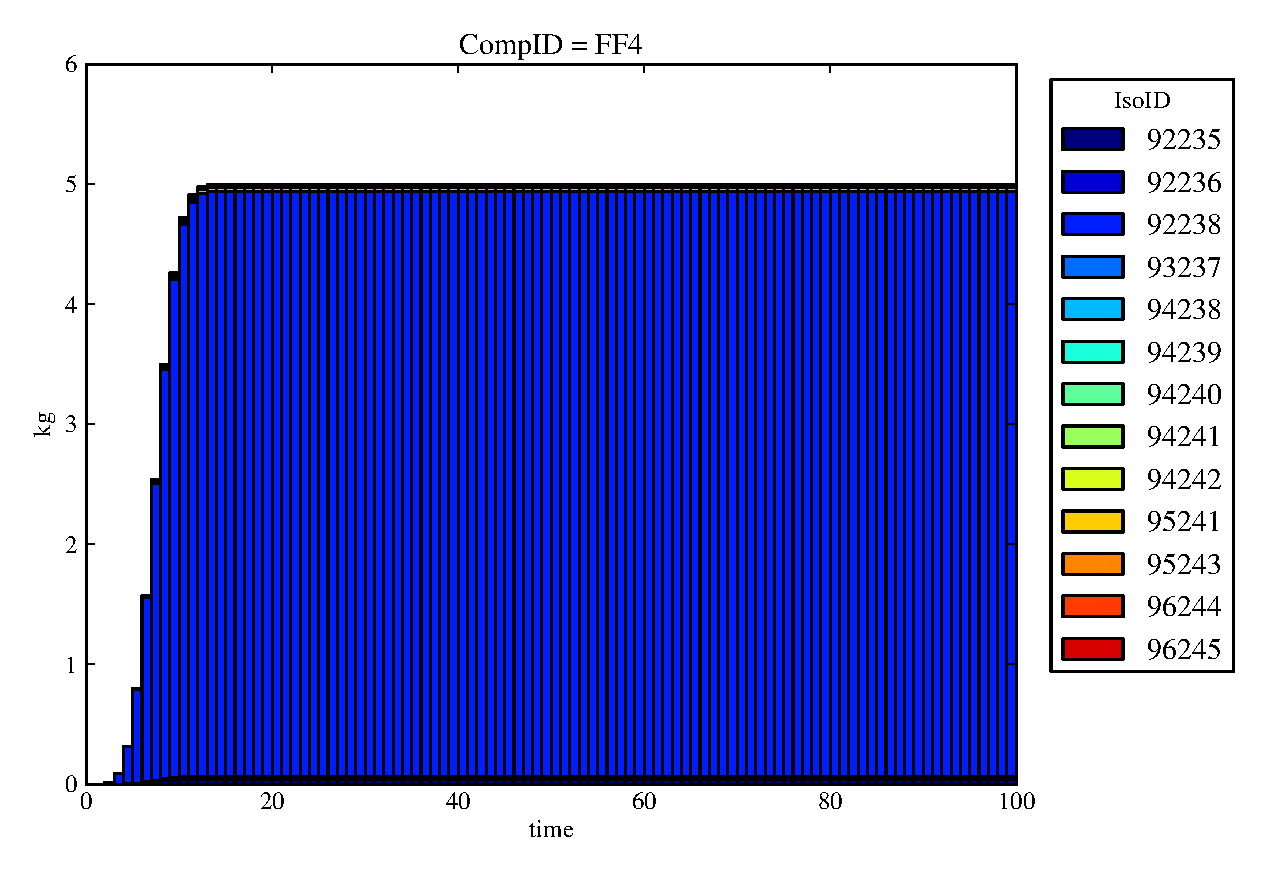
\includegraphics[width=\textwidth]{./chapters/demonstration/base/drIV0.eps}
  \caption[Case DRIII Waste Package Contaminants.]{ 
    The Far Field, component 0 ($F_d = 0.0$), acheives total containment.
    }
  \label{fig:drIVff0}


  \end{minipage}
\end{figure}

\FloatBarrier

\subsubsection{Mixed Cell Model}
The Mixed Cell model behaves similarly to the Degradation Rate model, when 
sorption and solubility limitation in that model are disabled (as in Figures 
\ref{fig:mcI} through \ref{fig:mcIff0}. When they are enabled, however, expected 
to demonstrate sorption limited and solubility limited transport as in Figures 
\ref{fig:mcIIIall} through \ref{fig:mcII}. The extent to which sorption and 
solubility limitation meet expectations is addressed in this base case.

Dual and single parameter verification cases were run to explore the effects of 
sorption and solubility limitation both separately and together.  Results from 
two of these base cases can be found in Figures \ref{fig:mcI} through 
\ref{fig:mcII}.
The fixed maximum transport mode was use between mixed cell components for speed 
and clarity of results.


\begin{frame}[ctb!]
  \frametitle{Mixed Cell Model Base Case I}
\begin{figure}[ht]
\centering
\includegraphics[width=0.8\textwidth]{./images/mcI.eps}
\caption[$^{235}U$ residence. Mixed Cell Sorption Limitation Without Solubility Limitation.]{
For the MCI case in which total containment is only is assumed in the far field, 
but sorption and solubility limitation neglected, demonstrates results exactly similar to 
DRIV, as expected.}
\label{fig:mcI}
\end{figure}
\end{frame}

\begin{frame}[ctb!]
  \frametitle{Mixed Cell Model Base Case I}
  \begin{figure}[htbp!]
\begin{minipage}[b]{0.45\linewidth}

  \includegraphics[width=\textwidth]{./images/mcI1.eps}
  \caption[MCI Waste Form Contaminants.]{
    Waste Form 5 ($F_d = 0.1$) releases material with degradation. 
    }
  \label{fig:mcIwf5}
  
  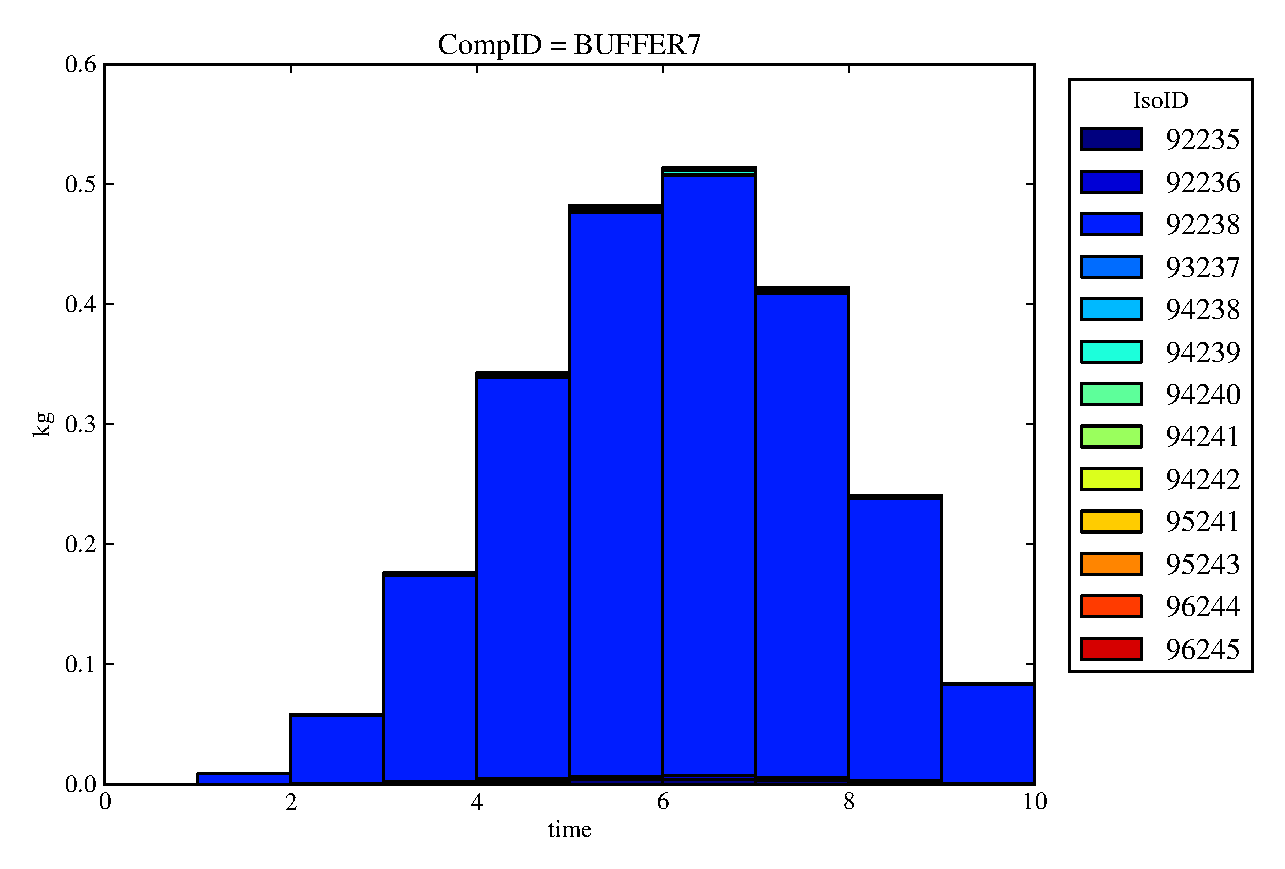
\includegraphics[width=\textwidth]{./images/mcI3.eps}
  \caption[Case MCI Buffer Contaminants]{
    The Buffer, component 7 ($F_d=0.1$), receives then releases material.
    }
  \label{fig:mcIbuff}

\end{minipage}
\hspace{0.05\linewidth}
\begin{minipage}[b]{0.45\linewidth}
  \includegraphics[width=\textwidth]{./images/mcI2.eps}
  \caption[Case MCI Waste Package Contaminants.]{ 
    Waste Package 6 ($F_d = 0.1$) recieves then releases material.
    }
  \label{fig:mcIwp6}

  \includegraphics[width=\textwidth]{./images/mcI0.eps}
  \caption[Case MCI Waste Package Contaminants.]{ 
    The Far Field, component 4 ($F_d = 0.0$), acheives full containment.
    }
  \label{fig:mcIff0}


  \end{minipage}
\end{figure}
\end{frame}

\begin{frame}[ctb!]
  \frametitle{Mixed Cell Model Base Case II}
\begin{figure}[ht]
\centering
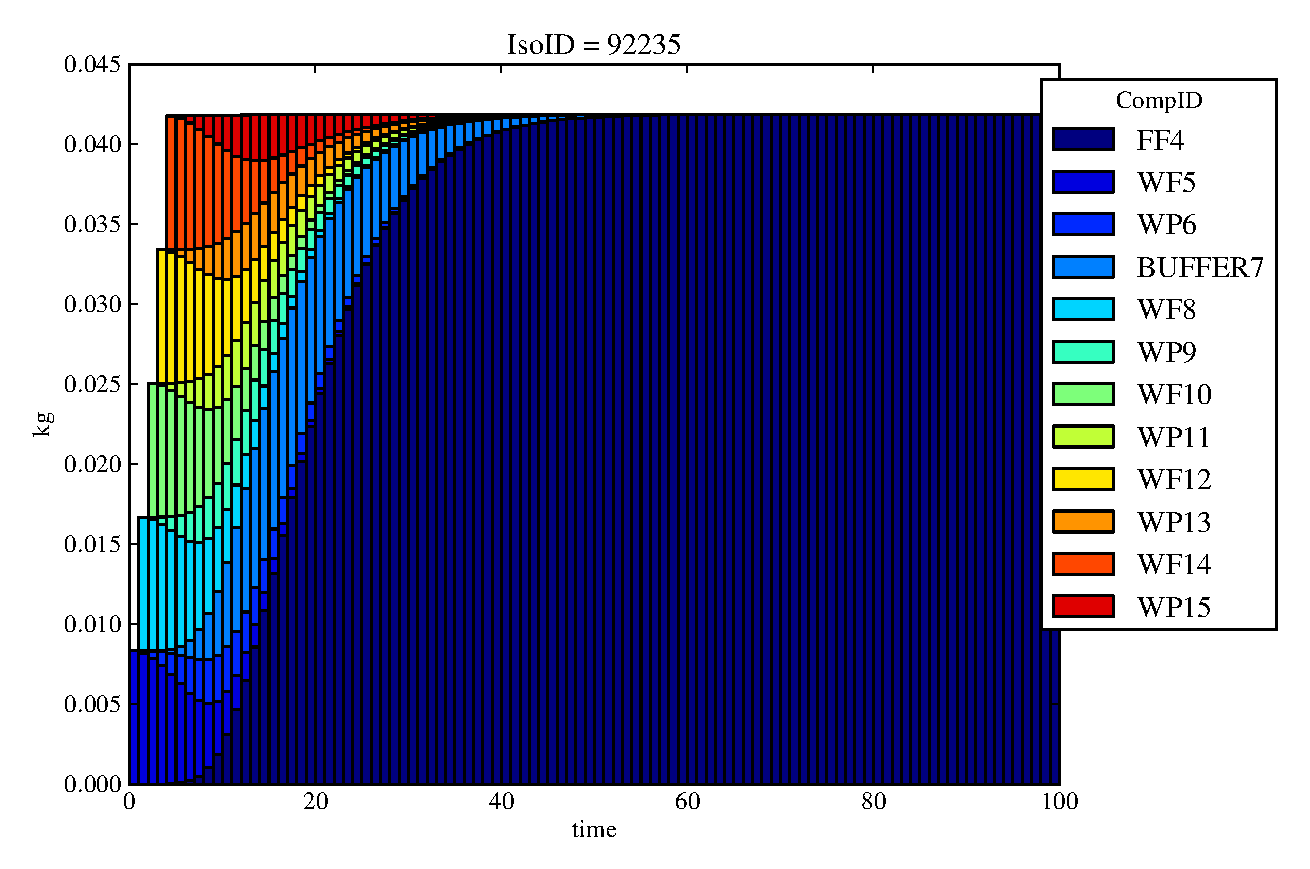
\includegraphics[width=0.8\textwidth]{./images/mcIII.eps}
\caption[$^{235}U$ residence. Mixed Cell Coupled Sorption and Solubility Limitation.]{
For the MCII case in which containment is affected by both sorption and 
solubility limitation,
($F_{d}=0.1$ for all components), $^{235}U$ travels more slowly than in the MCI case 
before permanent residence in the far field component.
}
\label{fig:mcIIIall}
\end{figure}
\end{frame}

\begin{frame}[ctb!]
  \frametitle{Mixed Cell Model Base Case II}
  \begin{figure}
\begin{minipage}[b]{0.45\linewidth}

  \includegraphics[width=\textwidth]{./images/mcIII1.eps}
  \caption[MCI Waste Form Contaminants.]{
    Waste Form 5 ($F_d = 0.1$) releases material with degradation. 
    }
  \label{fig:mcIIIwf5}
  
  \includegraphics[width=\textwidth]{./images/mcIII3.eps}
  \caption[Case MCI Buffer Contaminants]{
    The Buffer, component 7 ($F_d=0.1$), receives and then releases material.
    }
  \label{fig:mcIIIbuff}

\end{minipage}
\hspace{0.05\linewidth}
\begin{minipage}[b]{0.45\linewidth}
  \includegraphics[width=\textwidth]{./images/mcIII2.eps}
  \caption[Case MCI Waste Package Contaminants.]{ 
    Waste Package 6 ($F_d = 0.1$) recieves then releases material. 
    }
  \label{fig:mcIIIwp6}

  \includegraphics[width=\textwidth]{./images/mcIII0.eps}
  \caption[Case MCI Waste Package Contaminants.]{ 
    The Far Field, component 0 ($F_d = 0.1$), acheives total containment.
    }
  \label{fig:mcII}


  \end{minipage}
\end{figure}

\end{frame}

\FloatBarrier

\subsubsection{Lumped Parameter Model}
The Lumped Parameter model, with its three formulations (Exponential Model, 
Dispersion Model, and Piston flow Model) is not expected to receive 
contaminants if the porosity or advective velocity are zero. Else, however, 
contaminants are expected to  become available to the adjacent components 
according to the functional forms of the formulations. 

To observe the behaviors of each of the three formulations and to demonstrate 
full containment in cases where it is expected, simulations were run to 
investigate the impact of using various models. Results of these base cases can be found in Figures 
\ref{fig:lpBegin} through \ref{fig:lpEnd}.




\begin{figure}[ht]
\centering
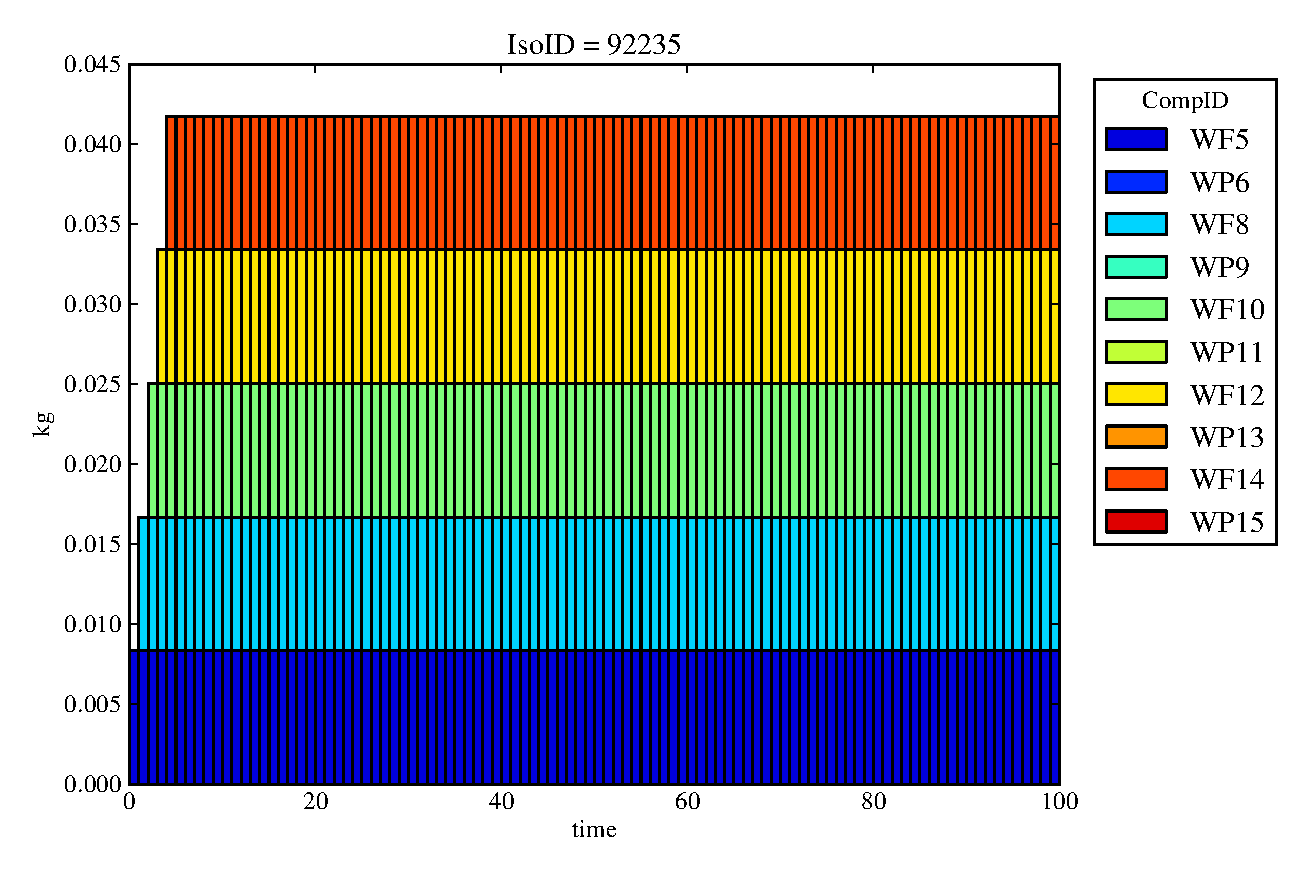
\includegraphics[width=0.6\textwidth]{./chapters/demonstration/base/lpEMII.eps}
\caption[$^{235}U$ residence. Lumped Parameter  Waste Package No Release.]{
For case LPEMII in which total containment in the waste package is assumed 
($F_{d,wp}=0$), $^{235}U$ travels through the waste form component ($F_d = 0.1$) before 
permanent residence in the waste package component.
}
\label{fig:lpBegin}
\begin{minipage}[b]{0.45\linewidth}

  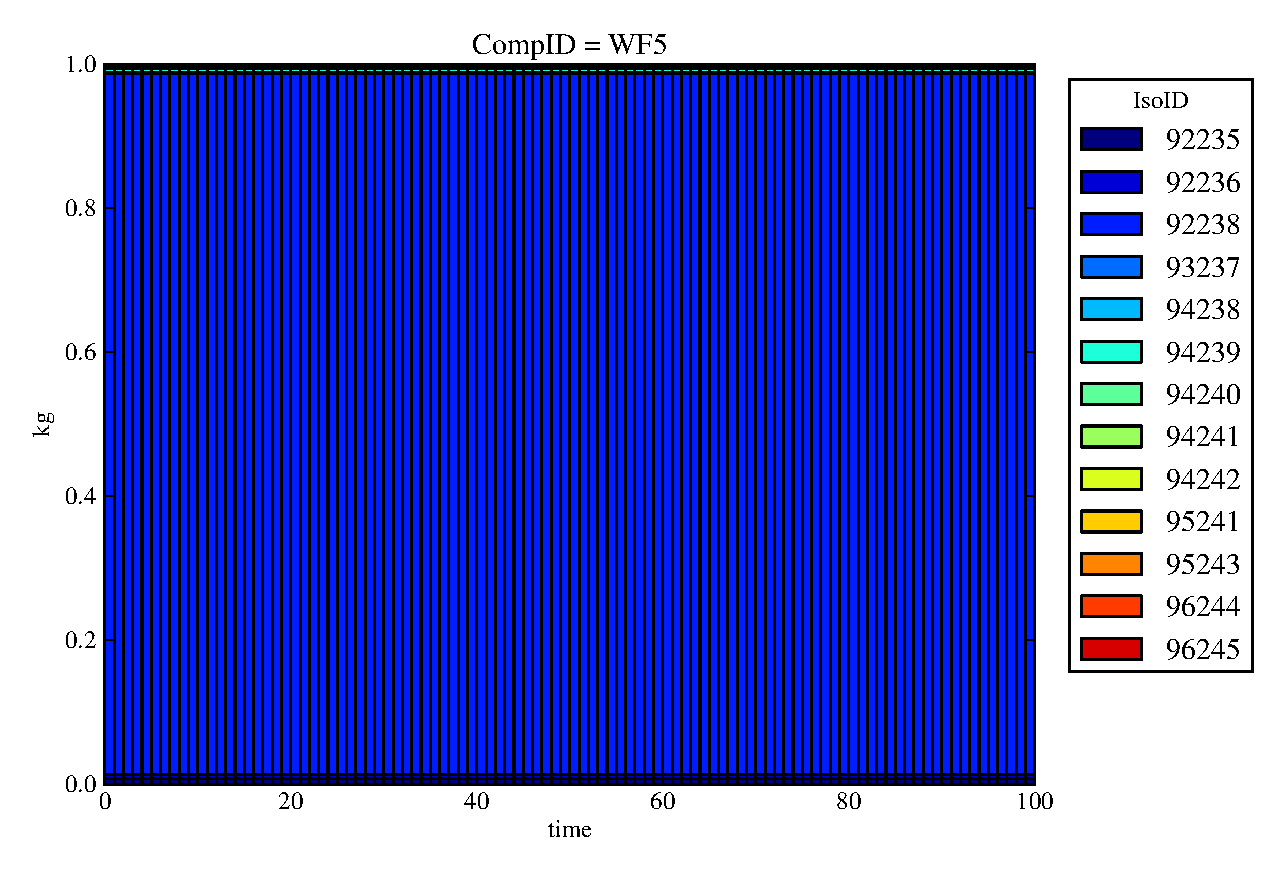
\includegraphics[width=\textwidth]{./chapters/demonstration/base/lpEMII1.eps}
  \caption[Case LPEMII Waste Form Contaminants.]{
    Waste Form 5 ($F_d = 0.1$) releases material with degradation. 
    }
  \label{fig:lpEMIIwf5}
  
  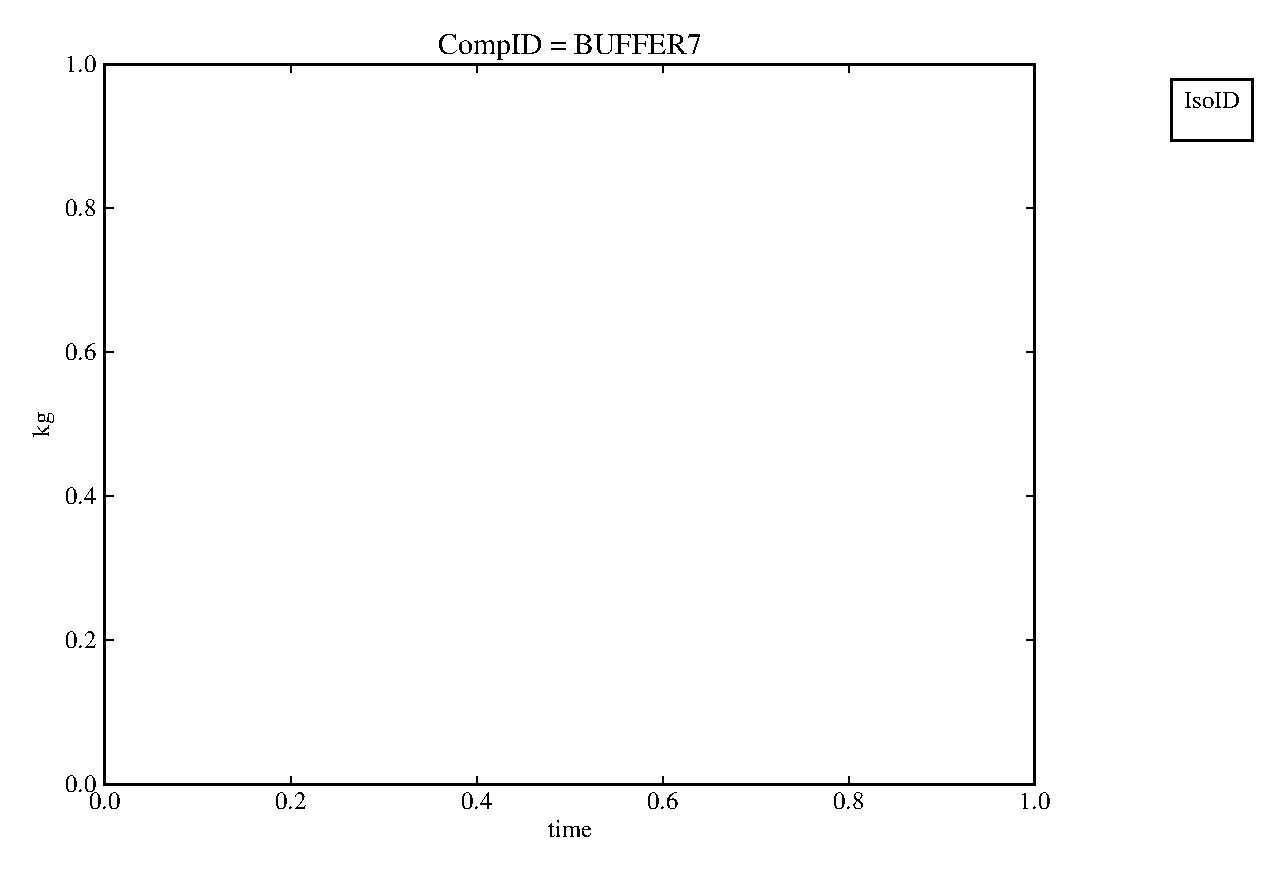
\includegraphics[width=\textwidth]{./chapters/demonstration/base/lpEMII3.eps}
  \caption[Case LPEMII Buffer Contaminants]{
    The Buffer, component 7 ($F_d=0.1$), never receives material.
    }
  \label{fig:lpEMIIbuff}

\end{minipage}
\hspace{0.05\linewidth}
\begin{minipage}[b]{0.45\linewidth}
  \includegraphics[width=\textwidth]{./chapters/demonstration/base/lpEMII2.eps}
  \caption[Case LPEMII Waste Package Contaminants.]{ 
    Waste Package 6 ($F_d = 0.0$) achieves total containment. 
    }
  \label{fig:lpEMIIwp6}

  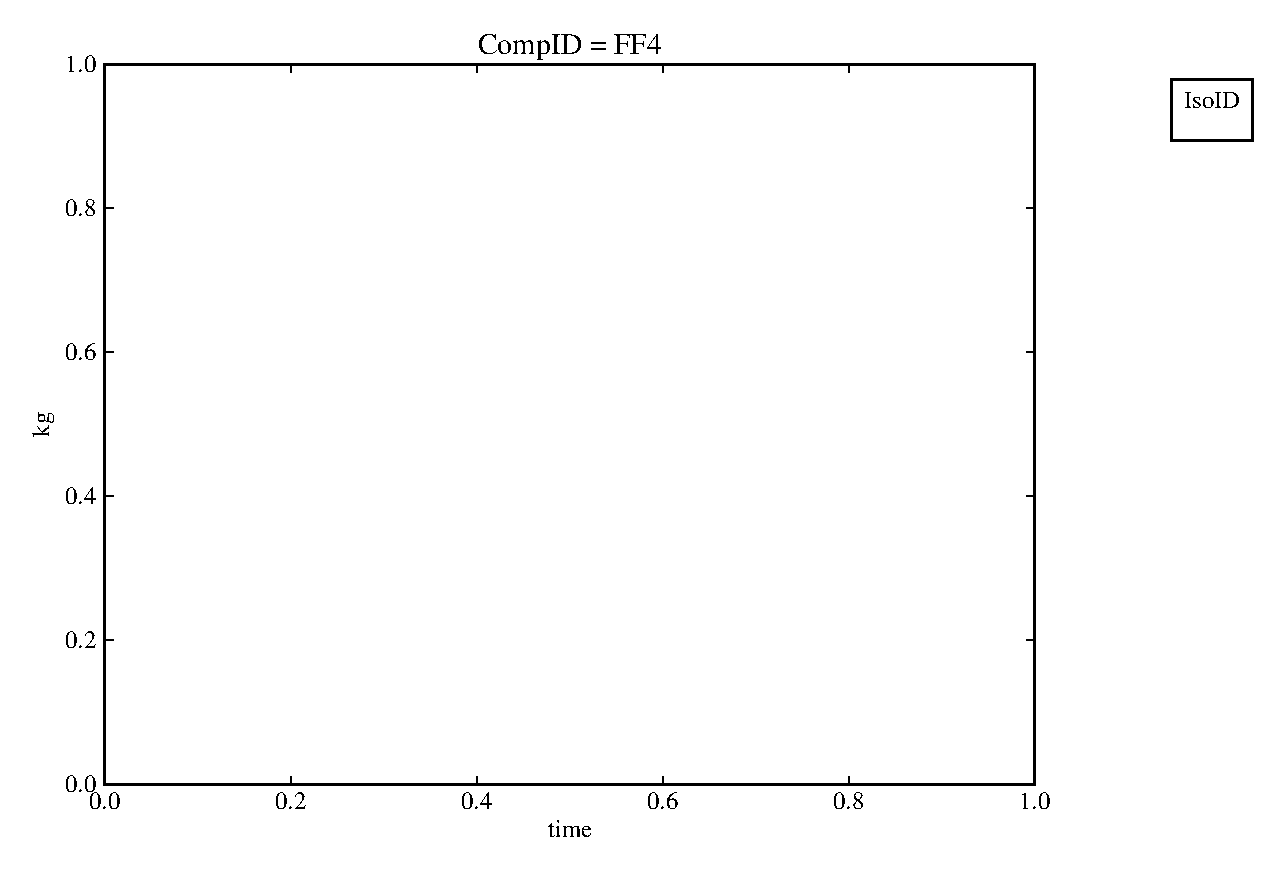
\includegraphics[width=\textwidth]{./chapters/demonstration/base/lpEMII0.eps}
  \caption[Case LPEMII Waste Package Contaminants.]{ 
    The Far Field, component 0 ($F_d = 0.1$), never receives material.
    }
  \label{fig:lpEMIIff0}


  \end{minipage}
\end{figure}


\begin{figure}[ht]
\centering
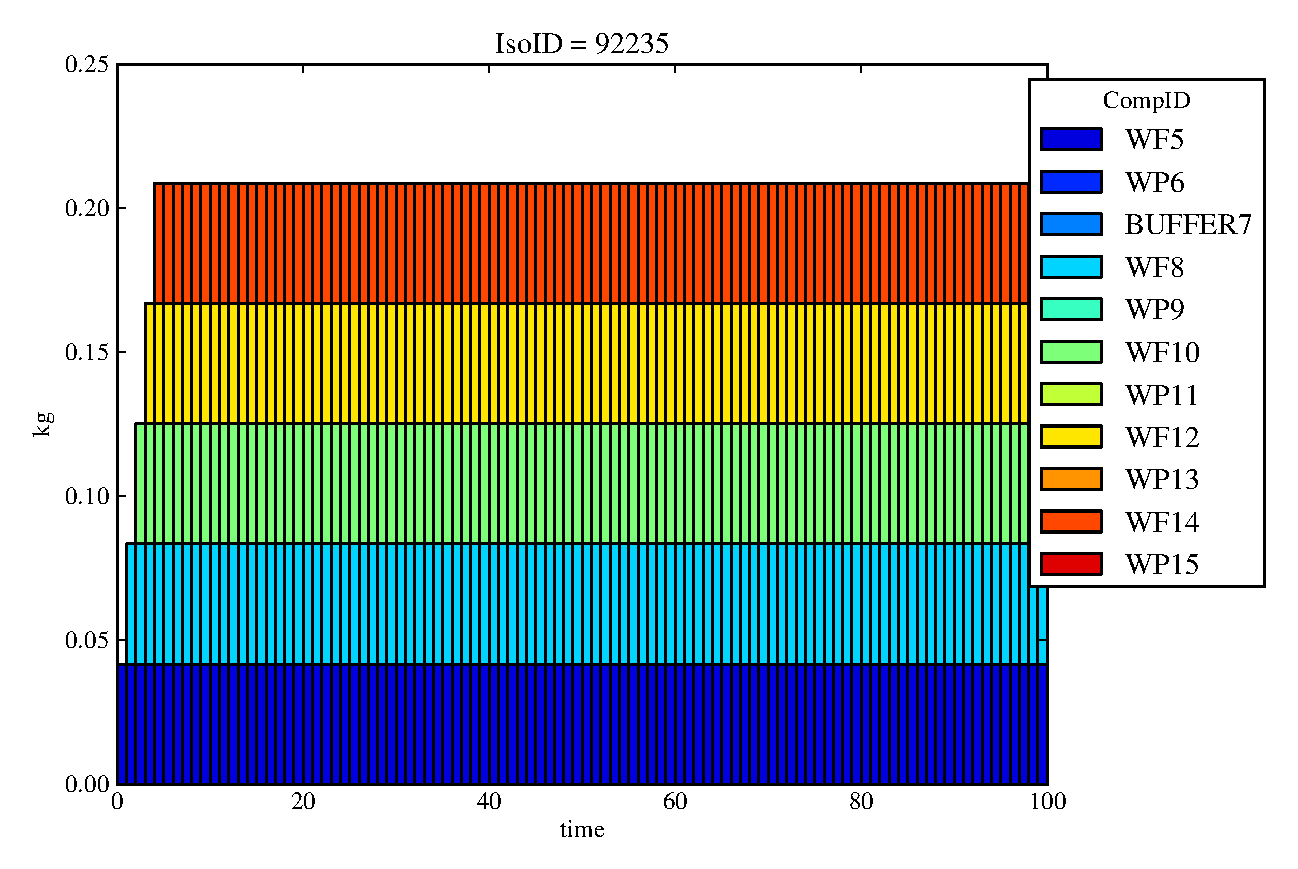
\includegraphics[width=0.6\textwidth]{./chapters/demonstration/base/lpDMII.eps}
\caption[$^{235}U$ residence. Lumped Parameter  DM Waste Package No Release.]{
For LPDMII case in which total containment in the waste package is assumed 
($F_{d,wp}=0$), $^{235}U$ travels through the waste form component ($F_d = 0.1$) before 
permanent residence in the waste package component.
}
\label{fig:lpDMIIall}
\begin{minipage}[b]{0.45\linewidth}

  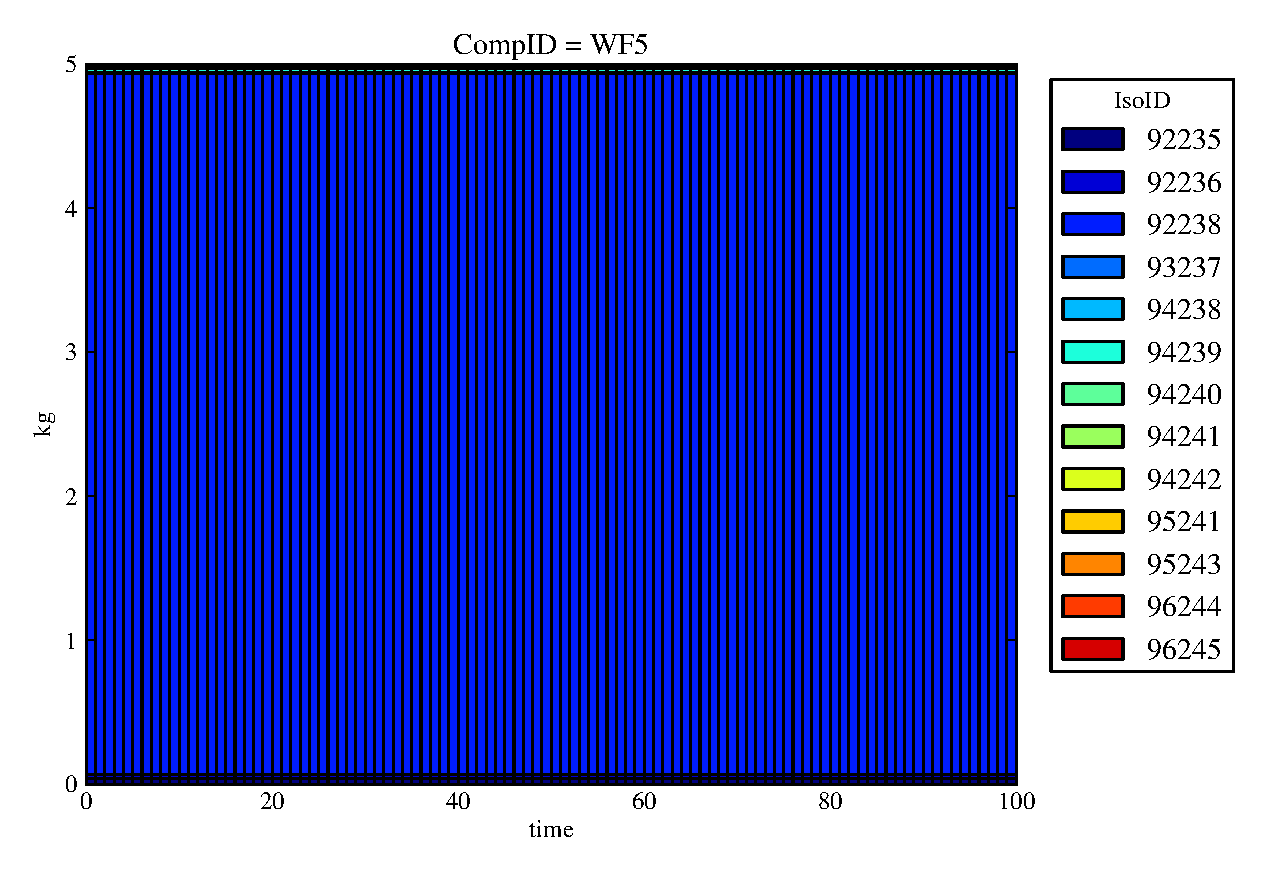
\includegraphics[width=\textwidth]{./chapters/demonstration/base/lpDMII1.eps}
  \caption[Case LPDMII Waste Form Contaminants.]{
    Waste Form 5 ($F_d = 0.1$) releases material with degradation. 
    }
  \label{fig:lpDMIIwf5}
  
  \includegraphics[width=\textwidth]{./chapters/demonstration/base/lpDMII3.eps}
  \caption[Case LPDMII Buffer Contaminants]{
    The Buffer, component 7 ($F_d=0.1$), never receives material.
    }
  \label{fig:lpDMIIbuff}

\end{minipage}
\hspace{0.05\linewidth}
\begin{minipage}[b]{0.45\linewidth}
  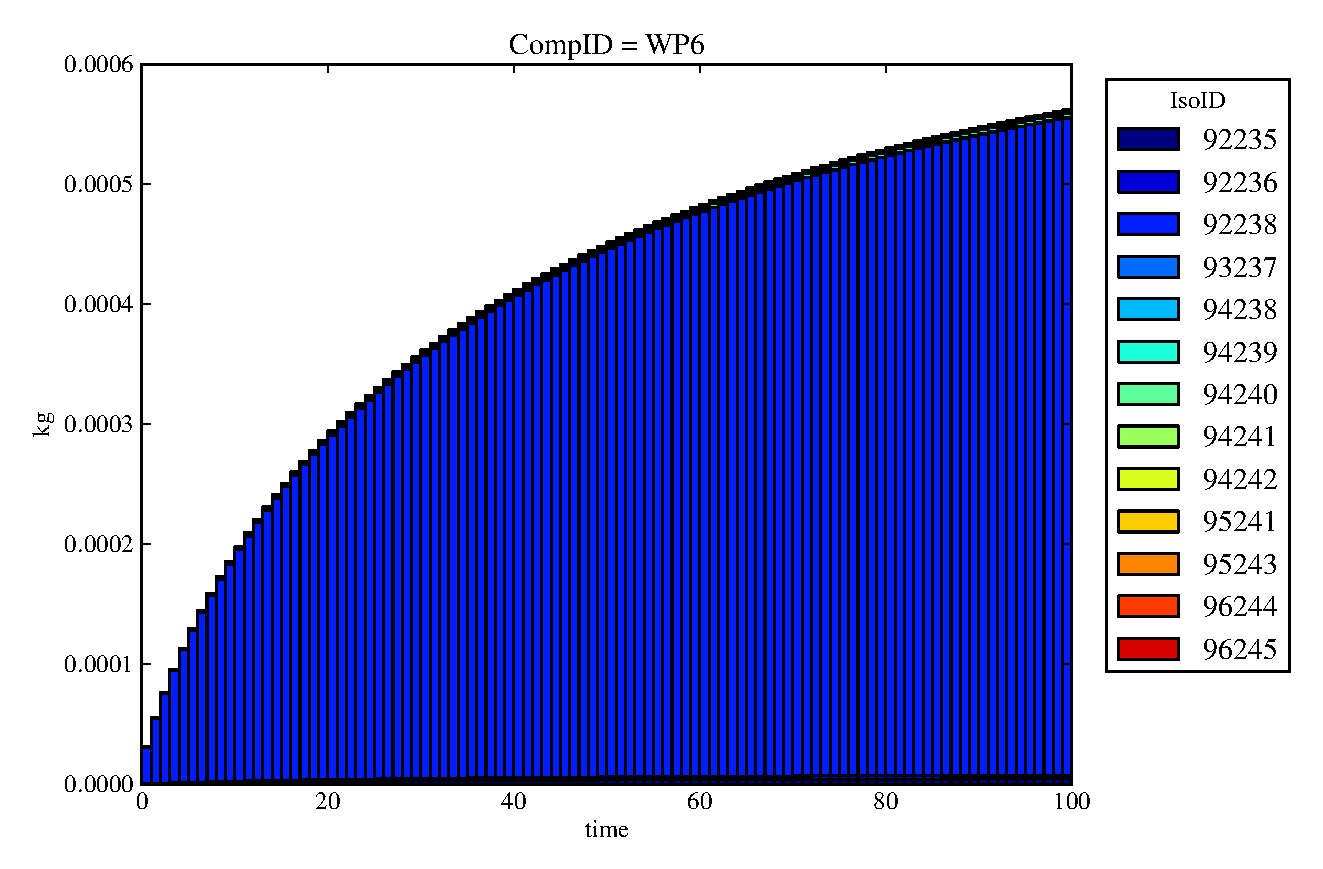
\includegraphics[width=\textwidth]{./chapters/demonstration/base/lpDMII2.eps}
  \caption[Case LPDMII Waste Package Contaminants.]{ 
    Waste Package 6 ($F_d = 0.0$) achieves total containment. 
    }
  \label{fig:lpDMIIwp6}

  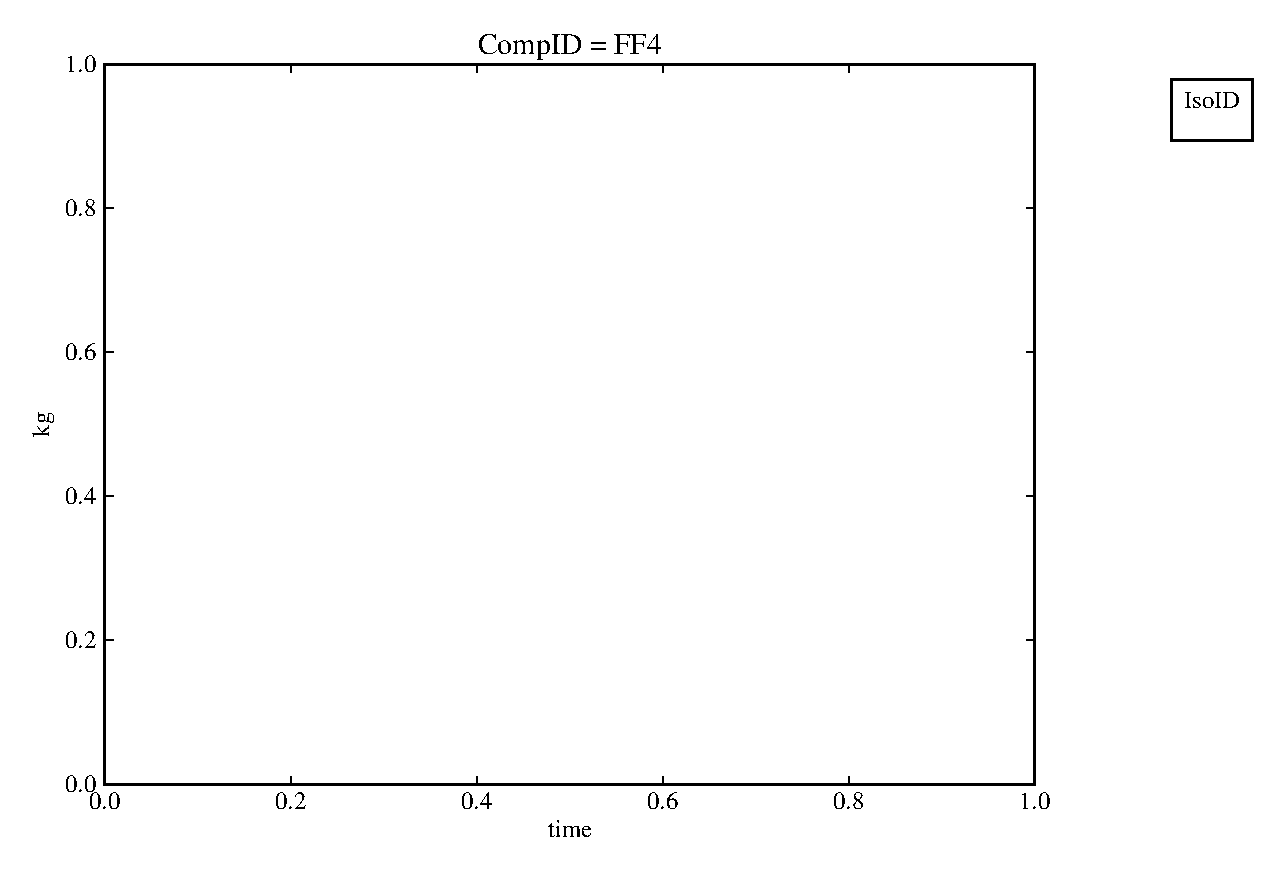
\includegraphics[width=\textwidth]{./chapters/demonstration/base/lpDMII0.eps}
  \caption[Case LPDMII Waste Package Contaminants.]{ 
    The Far Field, component 0 ($F_d = 0.1$), never receives material.
    }
  \label{fig:lpDMIIff0}


  \end{minipage}
\end{figure}

\begin{figure}[ht!]
\centering
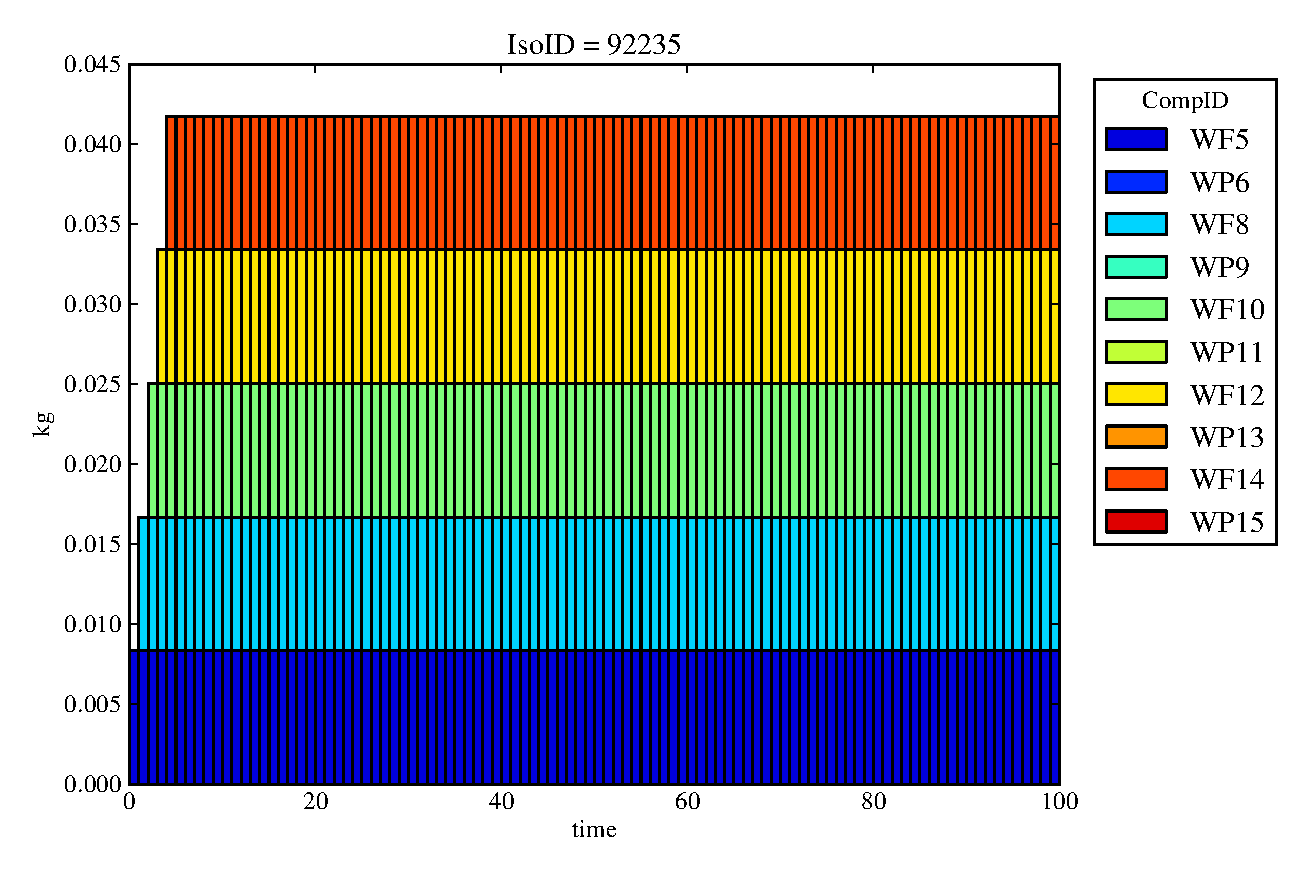
\includegraphics[width=0.6\textwidth]{./chapters/demonstration/base/lpPFMII.eps}
\caption[$^{235}U$ residence. Lumped Parameter PFM Waste Package No Release.]{
For case LPPFMII in which total containment in the waste package is assumed 
($F_{d,wp}=0$), $^{235}U$ travels through the waste form component ($F_d = 0.1$) before 
permanent residence in the waste package component.
}
\label{fig:lpPFMIIall}
\begin{minipage}[b]{0.45\linewidth}
  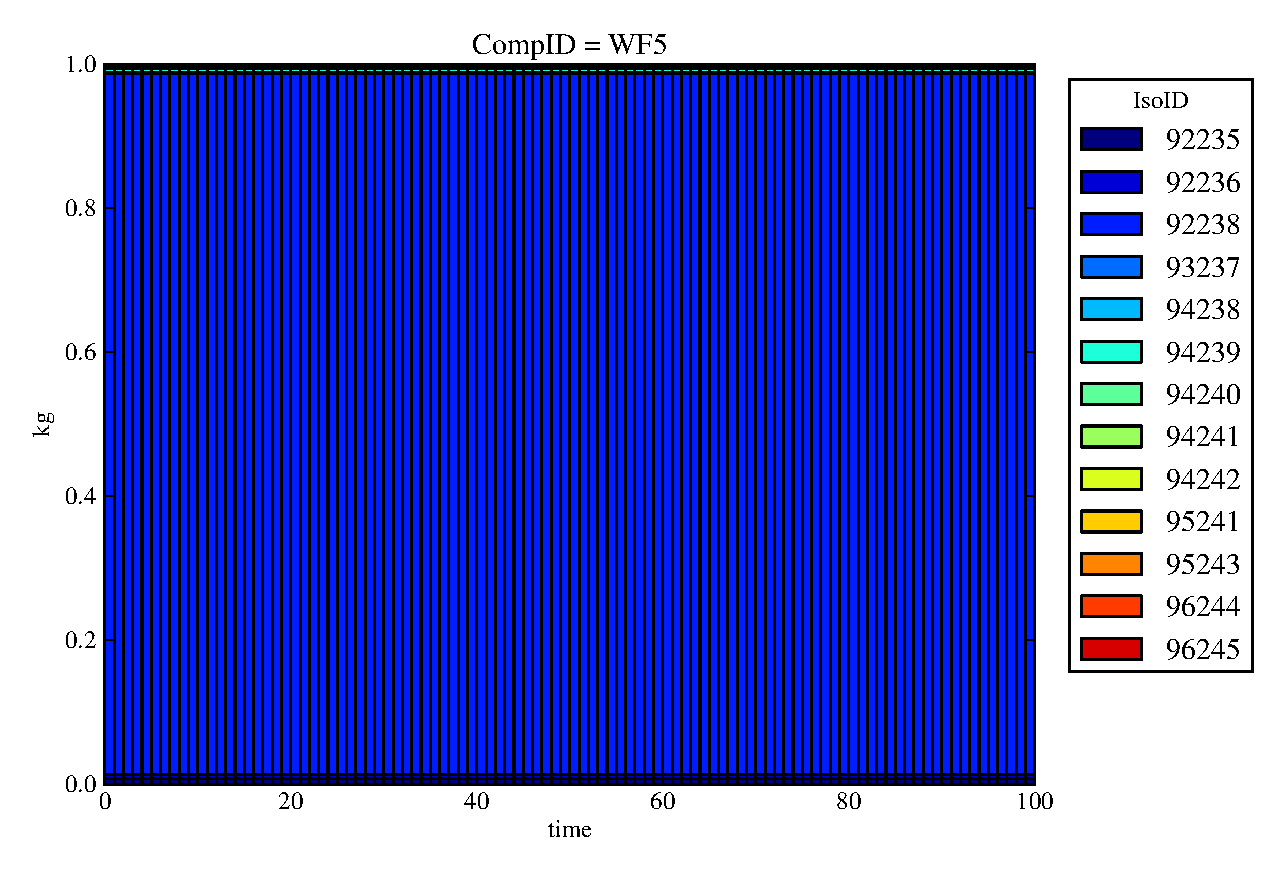
\includegraphics[width=\textwidth]{./chapters/demonstration/base/lpPFMII1.eps}
  \caption[Case LPPFMII Waste Form Contaminants.]{
    Waste Form 5 ($F_d = 0.1$) releases material with degradation. 
    }
  \label{fig:lpPFMIIwf5}
  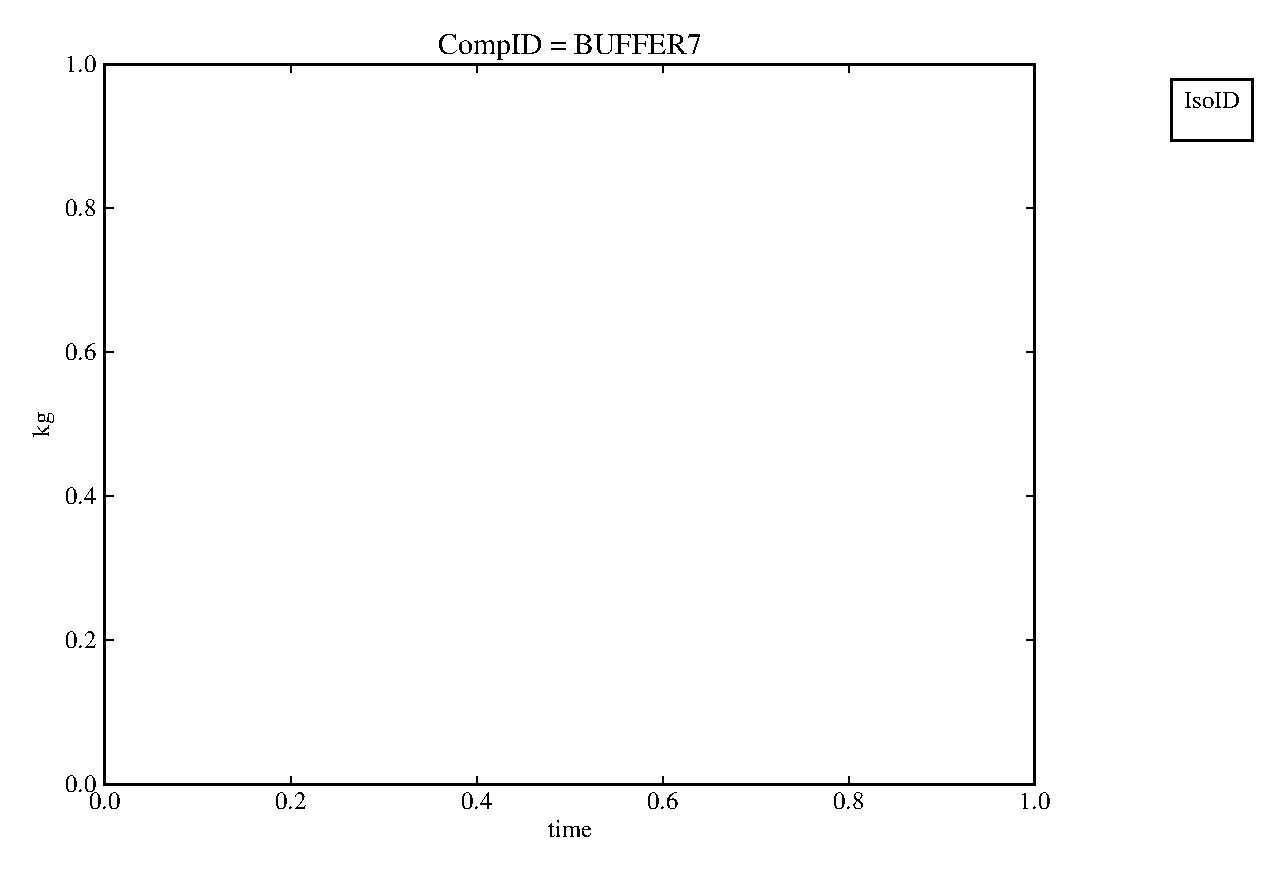
\includegraphics[width=\textwidth]{./chapters/demonstration/base/lpPFMII3.eps}
  \caption[Case LPPFMII Buffer Contaminants]{
    The Buffer, component 7 ($F_d=0$), never receives material.
    }
  \label{fig:lpPFMIIbuff}

\end{minipage}
\hspace{0.05\linewidth}
\begin{minipage}[b]{0.45\linewidth}
  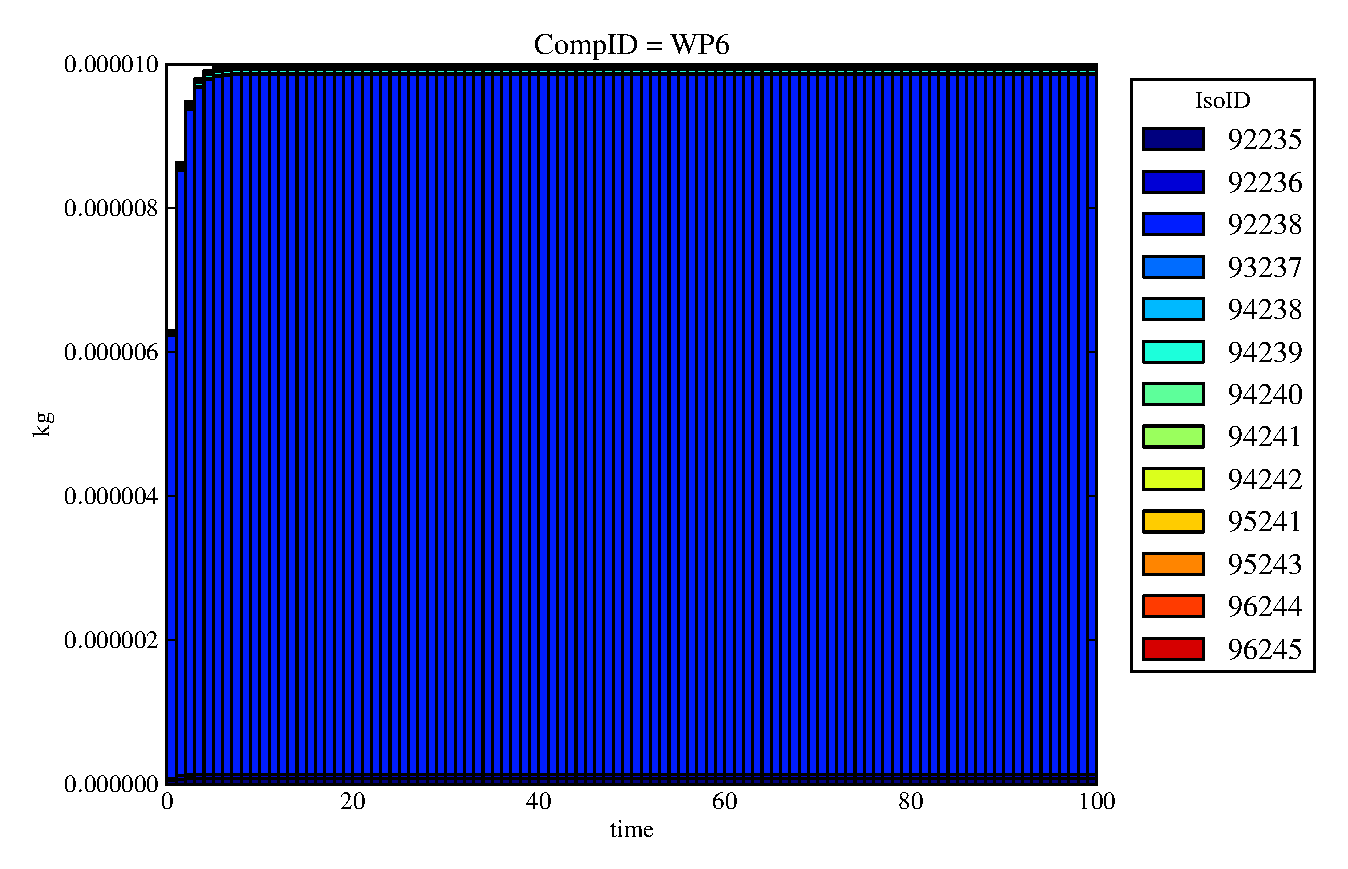
\includegraphics[width=\textwidth]{./chapters/demonstration/base/lpPFMII2.eps}
  \caption[Case LPPFMII Waste Package Contaminants.]{ 
    Waste Package 6 ($F_d = 0.1$) achieves total containment. 
    }
  \label{fig:lpPFMIIwp6}

  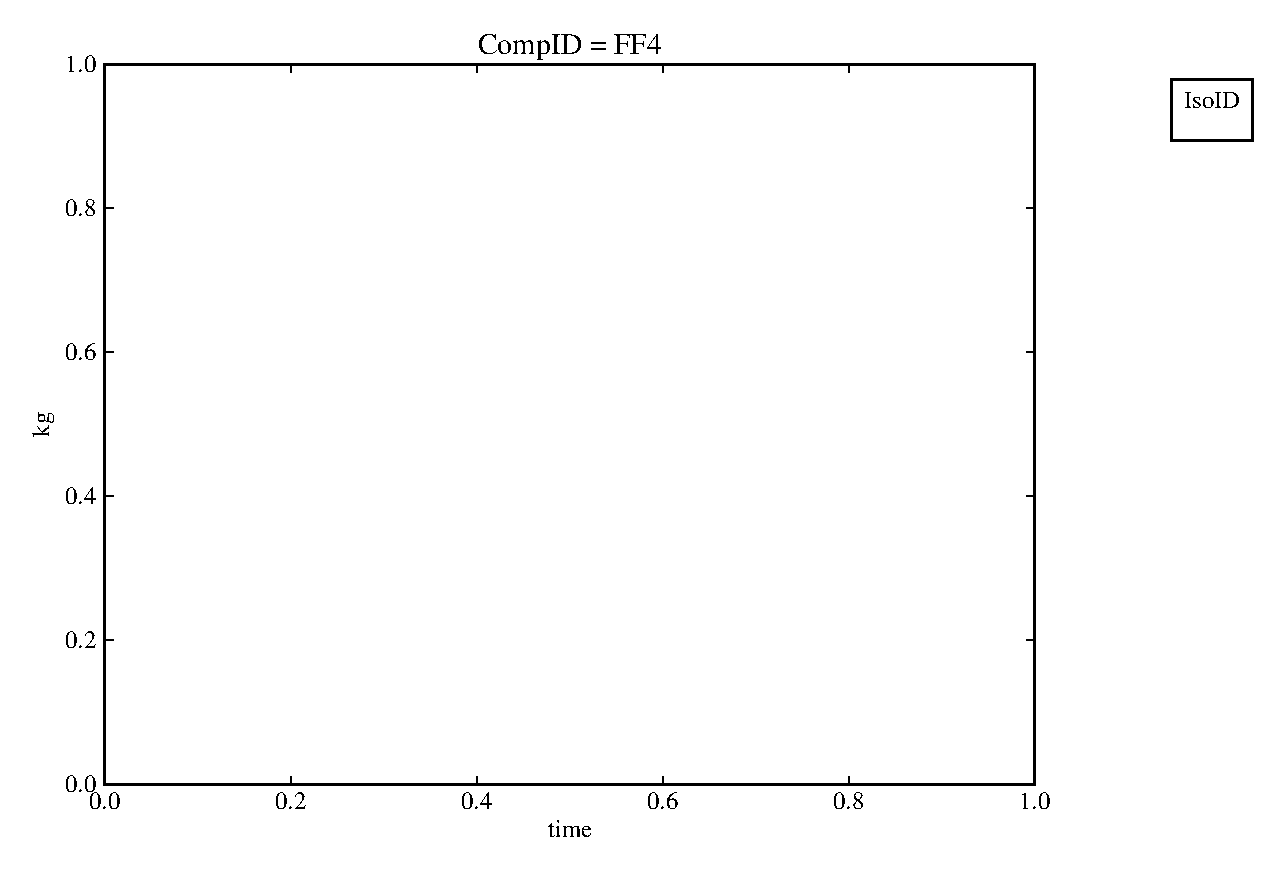
\includegraphics[width=\textwidth]{./chapters/demonstration/base/lpPFMII0.eps}
  \caption[Case LPPFMII Waste Package Contaminants.]{ 
    The Far Field, component 0 ($F_d = 0.1$), never receives material.
    }
  \label{fig:lpEnd}
  \end{minipage}
\end{figure} 
\FloatBarrier


The transit time that parameterizes these models could be based on radioactive 
tracer experiments in the field. Figures \ref{fig:lp_t_t_begin} 
and \ref{fig:lp_t_t_end} demonstrate the dependence of the resulting transport on 
transit time parameteriztion. These profiles demonstrate the trends seen in the 
analytical results demonstrated in Maloszewski and Zuber 
\cite{maloszewski_lumped_1996}.


\begin{frame}[ctb!]
  \frametitle{Dispersion Model} 
\begin{figure}[ht]
\centering
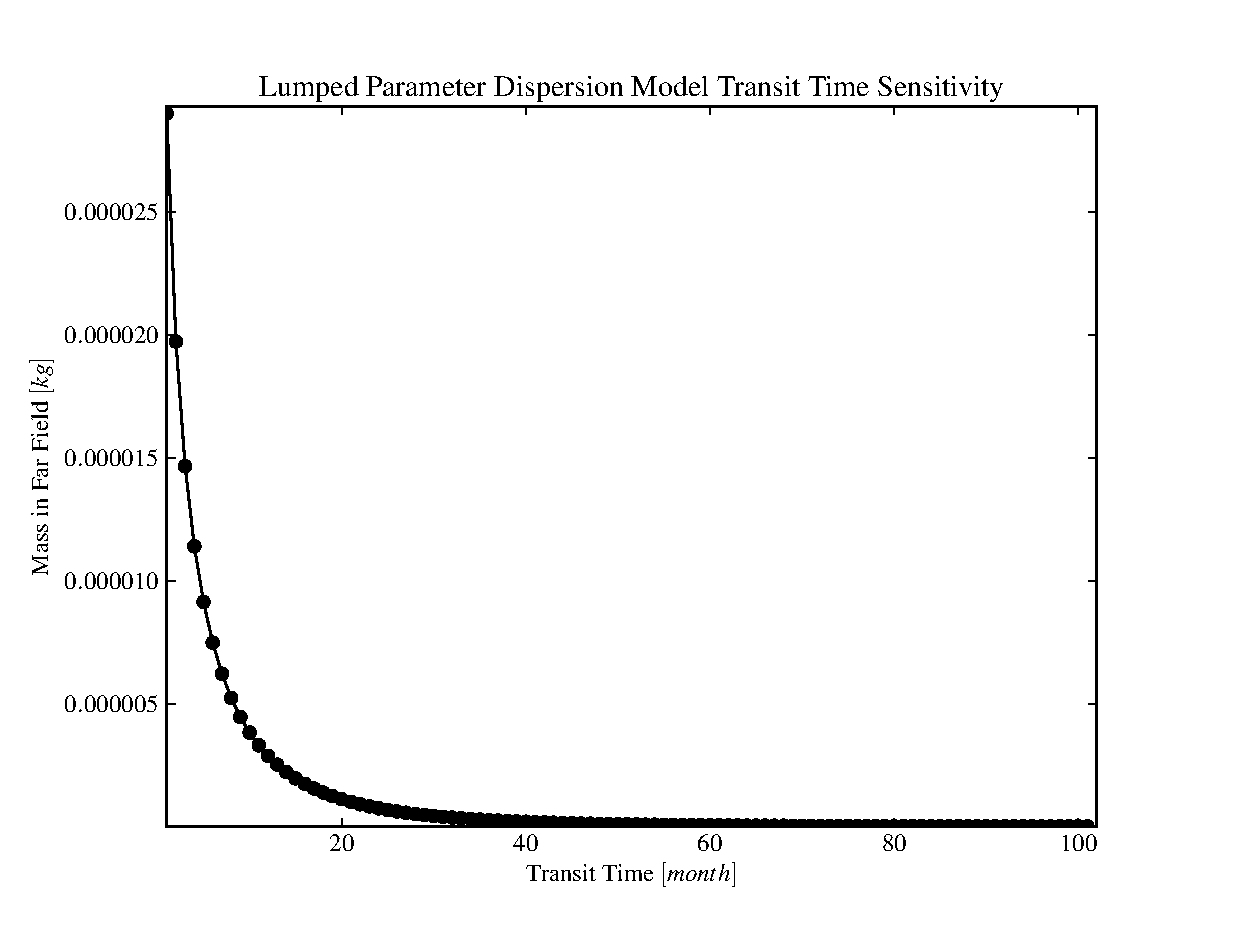
\includegraphics[width=0.8\textwidth]{./images/lpDM_t_t.eps}
\caption[Lumped Parameter Dispersion Model Transit Time Sensitivity]{The transit time 
parameterization of the lumped parameter dispersion model of radionuclide 
transport has a strong effect on the material reaching the far field after 30 
years.  }
\label{fig:lp_t_t_begin}
\end{figure}
\end{frame}


\begin{frame}[ctb!]
\frametitle{Exponential Model} 
\begin{figure}[ht]
\centering
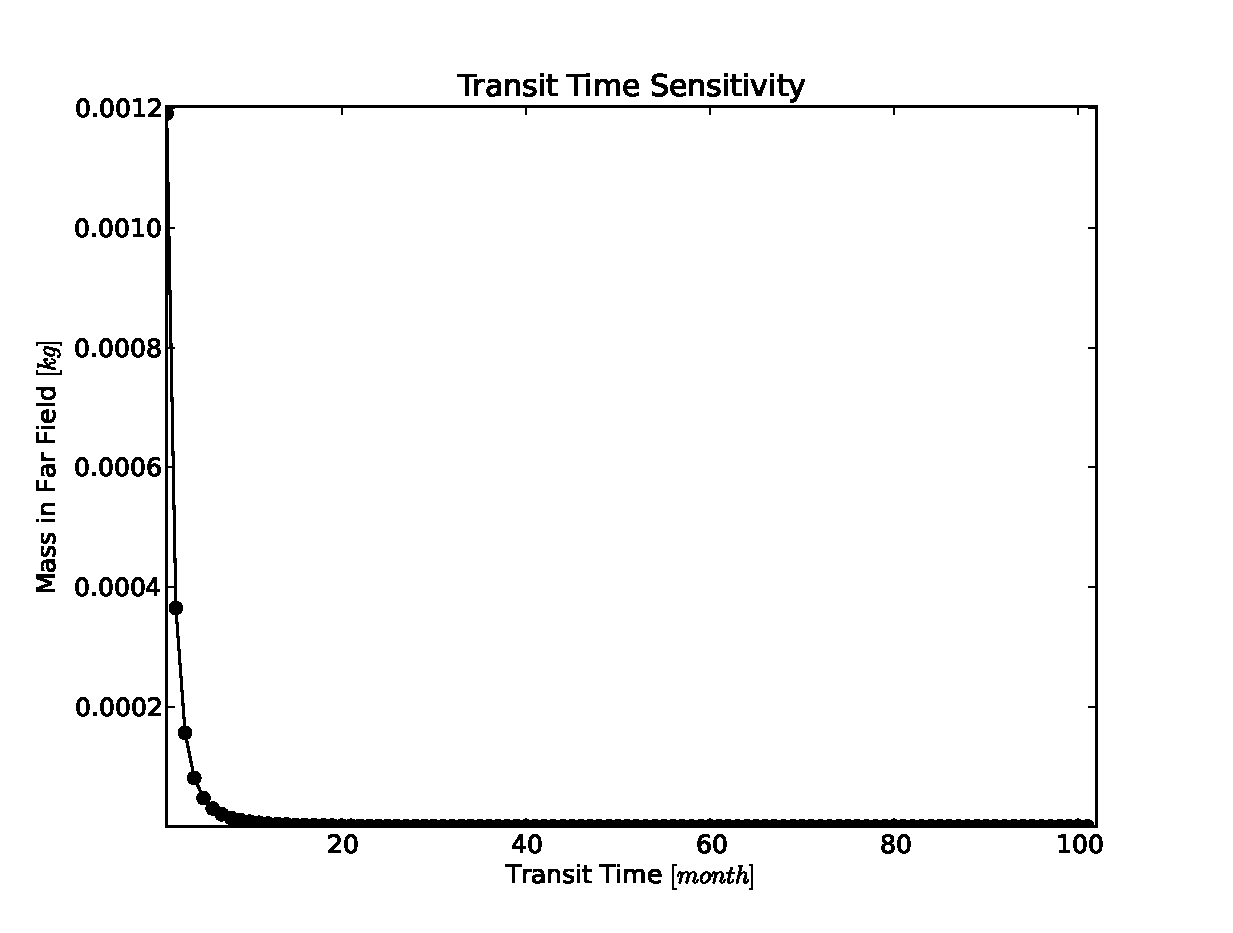
\includegraphics[width=0.8\textwidth]{./images/lpEXPM_t_t.eps}
\caption[Lumped Parameter Exponential Model Transit Time Sensitivity]{The transit time 
parameterization of the lumped parameter exponential model of radionuclide 
transport has a strong effect on the material reaching the far field after 30 
years.  }
\end{figure}
\end{frame}

\begin{frame}[ctb!]
\frametitle{Piston Flow Model} 
\begin{figure}[ht]
\centering
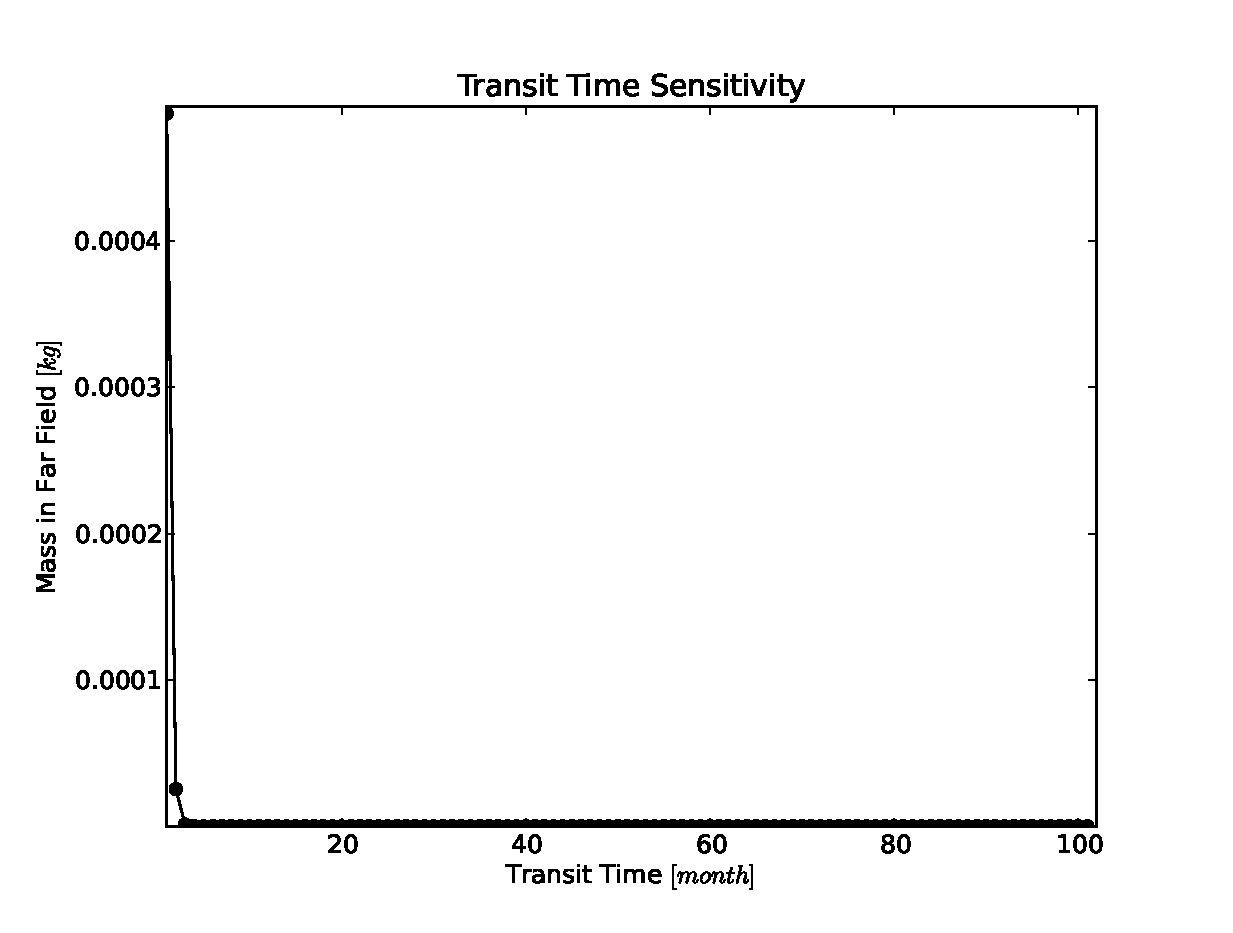
\includegraphics[width=0.8\textwidth]{./images/lpPFM_t_t.eps}
\caption[Lumped Parameter Piston Flow Model Transit Time Sensitivity]{The transit time 
parameterization of the lumped parameter piston flow model of radionuclide 
transport has a strong effect on the material reaching the far field after 30 
years.  }
\label{fig:lp_t_t_end}
\end{figure}

\end{frame}


\subsubsection{One Dimensional Permeable Porous Medium Model}
The One Dimensional PPM Model does not release contaminants if the porosity is 
zero or if both the reference diffusivity and advective velocity are zero. 
Else, however, contaminants are expected to  become available to the adjacent 
components according to the analytical form of the solution. The solution is 
only valid for advection and dispersion values within a realistic range, and 
the model accordingly can only be demonstrated for a very slow transport case. 

To observe the behavior of the solution and to demonstrate full containment in 
cases where it is expected, simulations were run with . An example simulation, with 
reference dispersion coefficient at $1\times 10^{-12}[m/s^2]$ and advective 
velocity of $1\times 10^{-15}$ [j] 
per waste form (to overwhelm numerical issues) is shown in Figure \ref{fig:odall}.  


\begin{figure}[ht]
\centering
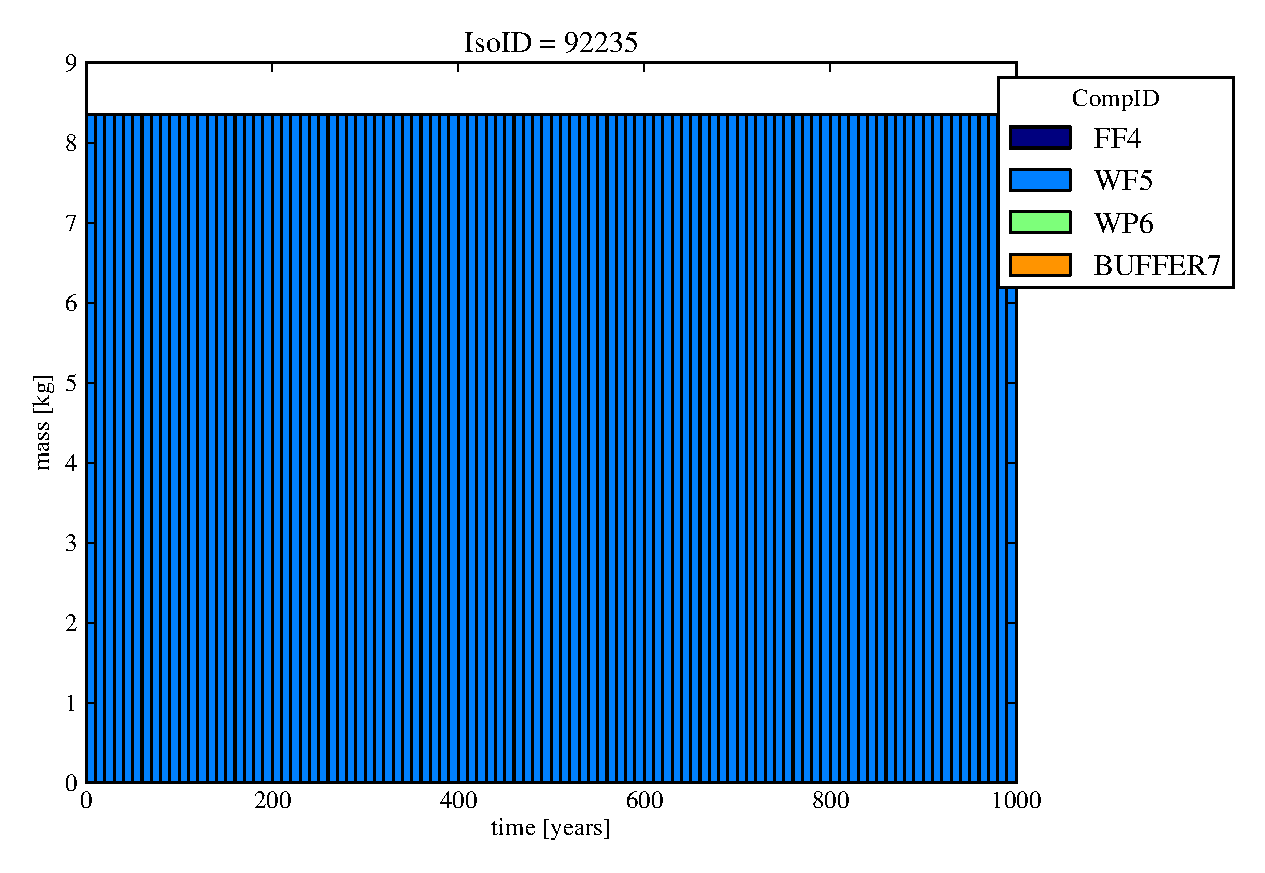
\includegraphics[width=0.6\textwidth]{./chapters/demonstration/base/od.eps}
\caption[One Dimensional PPM Model.]{
For the case in which transport through all components is represented by the 1 
Dimensional PPM model, material moves very slowly into the far field. 
}
\label{fig:odall}
\begin{minipage}[b]{0.45\linewidth}

  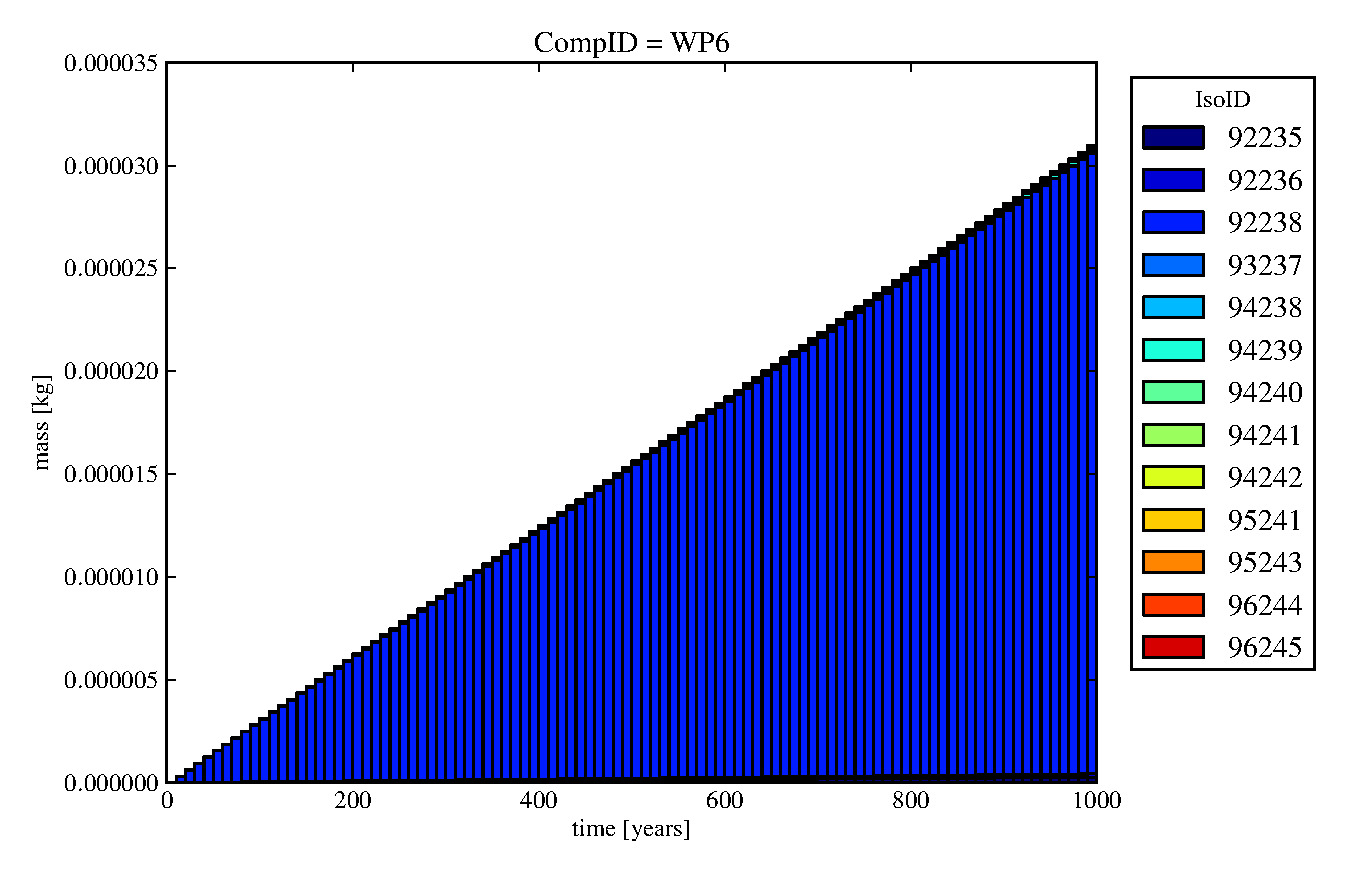
\includegraphics[width=\textwidth]{./chapters/demonstration/base/od2.eps}
  \caption[Case ODI Waste Form Contaminants.]{
    Waste Form 5 slowly releases material into Waste Package 6.
    }
  \label{fig:drIVwf5}
  \includegraphics[width=\textwidth]{./chapters/demonstration/base/od3.eps}
  \caption[Case ODI Buffer Contaminants]{
    The Buffer, component 7 very slowly receives then releases material.
    }
  \label{fig:drIVbuff}
\end{minipage}
\hspace{0.05\linewidth}
\begin{minipage}[b]{0.45\linewidth}
  \includegraphics[width=\textwidth]{./chapters/demonstration/base/od1.eps}
  \caption[Case ODI Waste Package Contaminants.]{ 
    Waste Package 6 very slowly receives then releases material. 
    }
  \label{fig:drIVwp6}
  \includegraphics[width=\textwidth]{./chapters/demonstration/base/od0.eps}
  \caption[Case ODI Waste Package Contaminants.]{ 
    All material is released into Far Field, component 4.
    }
  \label{fig:drIVff0}


  \end{minipage}
\end{figure}

\FloatBarrier
